% Options for packages loaded elsewhere
\PassOptionsToPackage{unicode}{hyperref}
\PassOptionsToPackage{hyphens}{url}
\PassOptionsToPackage{dvipsnames,svgnames,x11names}{xcolor}
%
\documentclass[
  letterpaper,
  DIV=11,
  numbers=noendperiod]{scrreprt}

\usepackage{amsmath,amssymb}
\usepackage{iftex}
\ifPDFTeX
  \usepackage[T1]{fontenc}
  \usepackage[utf8]{inputenc}
  \usepackage{textcomp} % provide euro and other symbols
\else % if luatex or xetex
  \usepackage{unicode-math}
  \defaultfontfeatures{Scale=MatchLowercase}
  \defaultfontfeatures[\rmfamily]{Ligatures=TeX,Scale=1}
\fi
\usepackage{lmodern}
\ifPDFTeX\else  
    % xetex/luatex font selection
\fi
% Use upquote if available, for straight quotes in verbatim environments
\IfFileExists{upquote.sty}{\usepackage{upquote}}{}
\IfFileExists{microtype.sty}{% use microtype if available
  \usepackage[]{microtype}
  \UseMicrotypeSet[protrusion]{basicmath} % disable protrusion for tt fonts
}{}
\makeatletter
\@ifundefined{KOMAClassName}{% if non-KOMA class
  \IfFileExists{parskip.sty}{%
    \usepackage{parskip}
  }{% else
    \setlength{\parindent}{0pt}
    \setlength{\parskip}{6pt plus 2pt minus 1pt}}
}{% if KOMA class
  \KOMAoptions{parskip=half}}
\makeatother
\usepackage{xcolor}
\setlength{\emergencystretch}{3em} % prevent overfull lines
\setcounter{secnumdepth}{-\maxdimen} % remove section numbering
% Make \paragraph and \subparagraph free-standing
\ifx\paragraph\undefined\else
  \let\oldparagraph\paragraph
  \renewcommand{\paragraph}[1]{\oldparagraph{#1}\mbox{}}
\fi
\ifx\subparagraph\undefined\else
  \let\oldsubparagraph\subparagraph
  \renewcommand{\subparagraph}[1]{\oldsubparagraph{#1}\mbox{}}
\fi


\providecommand{\tightlist}{%
  \setlength{\itemsep}{0pt}\setlength{\parskip}{0pt}}\usepackage{longtable,booktabs,array}
\usepackage{calc} % for calculating minipage widths
% Correct order of tables after \paragraph or \subparagraph
\usepackage{etoolbox}
\makeatletter
\patchcmd\longtable{\par}{\if@noskipsec\mbox{}\fi\par}{}{}
\makeatother
% Allow footnotes in longtable head/foot
\IfFileExists{footnotehyper.sty}{\usepackage{footnotehyper}}{\usepackage{footnote}}
\makesavenoteenv{longtable}
\usepackage{graphicx}
\makeatletter
\def\maxwidth{\ifdim\Gin@nat@width>\linewidth\linewidth\else\Gin@nat@width\fi}
\def\maxheight{\ifdim\Gin@nat@height>\textheight\textheight\else\Gin@nat@height\fi}
\makeatother
% Scale images if necessary, so that they will not overflow the page
% margins by default, and it is still possible to overwrite the defaults
% using explicit options in \includegraphics[width, height, ...]{}
\setkeys{Gin}{width=\maxwidth,height=\maxheight,keepaspectratio}
% Set default figure placement to htbp
\makeatletter
\def\fps@figure{htbp}
\makeatother
% definitions for citeproc citations
\NewDocumentCommand\citeproctext{}{}
\NewDocumentCommand\citeproc{mm}{%
  \begingroup\def\citeproctext{#2}\cite{#1}\endgroup}
\makeatletter
 % allow citations to break across lines
 \let\@cite@ofmt\@firstofone
 % avoid brackets around text for \cite:
 \def\@biblabel#1{}
 \def\@cite#1#2{{#1\if@tempswa , #2\fi}}
\makeatother
\newlength{\cslhangindent}
\setlength{\cslhangindent}{1.5em}
\newlength{\csllabelwidth}
\setlength{\csllabelwidth}{3em}
\newenvironment{CSLReferences}[2] % #1 hanging-indent, #2 entry-spacing
 {\begin{list}{}{%
  \setlength{\itemindent}{0pt}
  \setlength{\leftmargin}{0pt}
  \setlength{\parsep}{0pt}
  % turn on hanging indent if param 1 is 1
  \ifodd #1
   \setlength{\leftmargin}{\cslhangindent}
   \setlength{\itemindent}{-1\cslhangindent}
  \fi
  % set entry spacing
  \setlength{\itemsep}{#2\baselineskip}}}
 {\end{list}}
\usepackage{calc}
\newcommand{\CSLBlock}[1]{\hfill\break\parbox[t]{\linewidth}{\strut\ignorespaces#1\strut}}
\newcommand{\CSLLeftMargin}[1]{\parbox[t]{\csllabelwidth}{\strut#1\strut}}
\newcommand{\CSLRightInline}[1]{\parbox[t]{\linewidth - \csllabelwidth}{\strut#1\strut}}
\newcommand{\CSLIndent}[1]{\hspace{\cslhangindent}#1}

\KOMAoption{captions}{tableheading}
\makeatletter
\@ifpackageloaded{bookmark}{}{\usepackage{bookmark}}
\makeatother
\makeatletter
\@ifpackageloaded{caption}{}{\usepackage{caption}}
\AtBeginDocument{%
\ifdefined\contentsname
  \renewcommand*\contentsname{Table of contents}
\else
  \newcommand\contentsname{Table of contents}
\fi
\ifdefined\listfigurename
  \renewcommand*\listfigurename{List of Figures}
\else
  \newcommand\listfigurename{List of Figures}
\fi
\ifdefined\listtablename
  \renewcommand*\listtablename{List of Tables}
\else
  \newcommand\listtablename{List of Tables}
\fi
\ifdefined\figurename
  \renewcommand*\figurename{Figure}
\else
  \newcommand\figurename{Figure}
\fi
\ifdefined\tablename
  \renewcommand*\tablename{Table}
\else
  \newcommand\tablename{Table}
\fi
}
\@ifpackageloaded{float}{}{\usepackage{float}}
\floatstyle{ruled}
\@ifundefined{c@chapter}{\newfloat{codelisting}{h}{lop}}{\newfloat{codelisting}{h}{lop}[chapter]}
\floatname{codelisting}{Listing}
\newcommand*\listoflistings{\listof{codelisting}{List of Listings}}
\makeatother
\makeatletter
\makeatother
\makeatletter
\@ifpackageloaded{caption}{}{\usepackage{caption}}
\@ifpackageloaded{subcaption}{}{\usepackage{subcaption}}
\makeatother
\ifLuaTeX
  \usepackage{selnolig}  % disable illegal ligatures
\fi
\usepackage{bookmark}

\IfFileExists{xurl.sty}{\usepackage{xurl}}{} % add URL line breaks if available
\urlstyle{same} % disable monospaced font for URLs
\hypersetup{
  pdftitle={FMA A-Team Manual},
  pdfauthor={Analytical Services Fisheries Monitoring and Analaysis AFSC, NOAA Fisheries},
  colorlinks=true,
  linkcolor={blue},
  filecolor={Maroon},
  citecolor={Blue},
  urlcolor={Blue},
  pdfcreator={LaTeX via pandoc}}

\title{FMA A-Team Manual}
\author{Analytical Services\\
Fisheries Monitoring and Analaysis\\
AFSC, NOAA Fisheries}
\date{2024-07-01}

\begin{document}
\maketitle

\renewcommand*\contentsname{Table of contents}
{
\hypersetup{linkcolor=}
\setcounter{tocdepth}{2}
\tableofcontents
}
\bookmarksetup{startatroot}

\chapter[Welcome!]{\texorpdfstring{Welcome!\footnote{This manual is a
  collaborative effort of the FMA A-Team, with input from AFSC FMA
  Division staff.}}{Welcome!}}\label{welcome}

This is the manual for the Analytical Services Program in the Fisheries
Monitoring and Analysis Division at NOAA's Alaska Fisheries Science
Center\footnote{Jeepers, that's a mouthful! Let's just abbreviate from
  now on - acronym definitions are \hyperref[sec-acronyms]{here}}.

FMA's Analytical Services Program provides scientific products to
support the management of marine ecosystems and commercial fisheries.

This manual is intended to provide an overview for Program staff and
others about how we do our work, and our expectations. It is also a
space to document institutional knowledge and for important information
about procedures and available resources. If you have suggestions for
additions or changes, please contact the Analytical Services Program
Manager, Jason Jannot (jason /dot/ jannot /at/ noaa /dot/ gov).
Alternatively you can
\href{https://github.com/jjannot-NOAA/ateam-manual}{make a pull request,
or submit an issue to the Github repo}.

\bookmarksetup{startatroot}

\chapter{Introduction}\label{intro}

The FMA Analytical Services Program adheres to NOAA's mission of
\href{https://www.noaa.gov/our-mission-and-vision}{Science, Service, and
Stewardship}.

Background on the history, science, and management of Alaska fisheries
and the North Pacific Observer Program can be found in
\href{fishery-background.qmd}{Appendix A - Alaska Fisheries Background}

In short, the mission of the Analytical Services Program is to use
fishery-dependent data collected by the FMA, in conjunction with other
data sources collected by various agencies, to create scientific
products that inform fisheries management and science.

\hyperref[sec-big_picture]{The Big Picture} describes our culture and
philosophy in more detail.

The FMA Analytical Services Program was a team for many years prior to
becoming a fully-fledged program in May 2023. Internally, we informally
refer to ourselves as the A-Team.

\section{Who We Are}\label{who-we-are}

As of 2024, the Analytical Services Program consists of

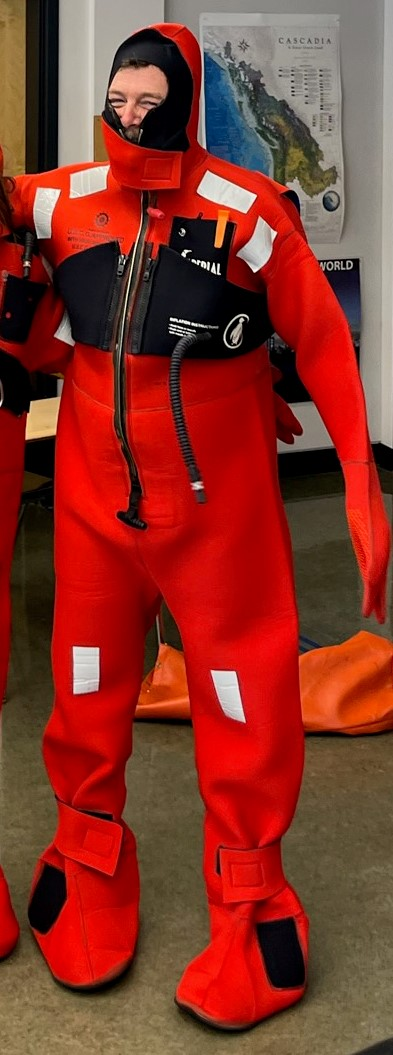
\includegraphics[width=\textwidth,height=3.125in]{_img/JJ_immersionsuit.jpg}

\href{https://www.fisheries.noaa.gov/contact/jason-e-jannot}{\textbf{Jason
Jannot, Program Manager}}\\
Supervisory Research Fishery Biologist (NMFS)\\
AFSC, Seattle\\
pronouns: he/him/his

Jason was originally hired as an analyst with the FMA A-Team in February
2023 and became the PM in May 2023. Jason worked as a data analyst for
the West Coast Groundfish and At-Sea Hake Observer Programs from
2010-2022 and for the International Pacific Halibut Commission from
2022-23.

\textbf{Interests}

\begin{itemize}
\tightlist
\item
  professional: leadership, team building, program management, project
  management, succession planning\\
\item
  personal: biking, bluegrass banjo, telemark skiing, travel, books,
  painting, German language
\end{itemize}

Learn more about his leadership style \href{jjphilosophy.qmd}{here} and
about him at his personal \href{https://jjannot.github.io/}{website}.

\begin{center}\rule{0.5\linewidth}{0.5pt}\end{center}

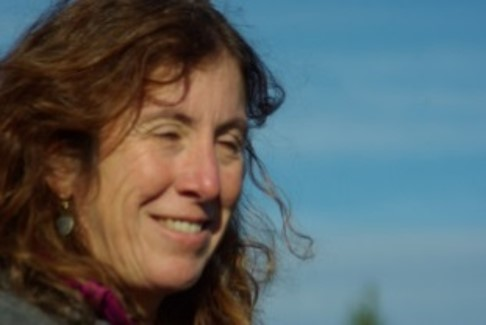
\includegraphics[width=\textwidth,height=1.5625in]{_img/JenCahalan.jpg}

\textbf{Jennifer Cahalan, Statistician}\\
Pacific States Marine Fisheries Commission\\
AFSC, Seattle

\textbf{Interests}

\begin{itemize}
\tightlist
\item
  professional: statistics, sampling design, estimation
\end{itemize}

\begin{center}\rule{0.5\linewidth}{0.5pt}\end{center}

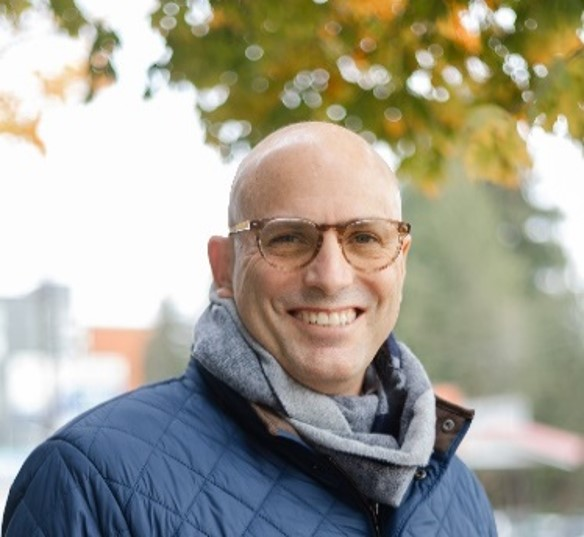
\includegraphics[width=\textwidth,height=1.5625in]{_img/CraigFaunce.jpg}

\textbf{Craig Faunce, Data Analyst}\\
Research Fish Biologist (NMFS)\\
AFSC, Seattle

\textbf{Interests}

\begin{itemize}
\tightlist
\item
  professional: observer effects, annual deployment plans, project
  management\\
\item
  personal: sports, nature, music, family
\end{itemize}

You can learn more about Craig,
\href{https://www.fisheries.noaa.gov/contact/craig-h-faunce}{here}

\begin{center}\rule{0.5\linewidth}{0.5pt}\end{center}


\includegraphics[width=\textwidth,height=1.5625in]{_img/ChristianGredzens.jpg}

\textbf{Christian Gredzens, Data Analyst}\\
Research Fish Biologist (NMFS)\\
AFSC, Seattle

\textbf{Interests}

\begin{itemize}
\tightlist
\item
  professional: spatial analyses\\
\item
  personal: reading, outdoors, biking, diving
\end{itemize}

\begin{center}\rule{0.5\linewidth}{0.5pt}\end{center}


\includegraphics[width=\textwidth,height=2.08333in]{_img/AndyKingham.jpg}

\textbf{Andy Kingham, Data Analyst \& Developer}\\
Operations Research Analyst (NMFS)\\
AFSC, Seattle

\textbf{Interests}

\begin{itemize}
\tightlist
\item
  professional: database and application development, operations\\
\item
  personal: sports, fishing, family
\end{itemize}

\begin{center}\rule{0.5\linewidth}{0.5pt}\end{center}

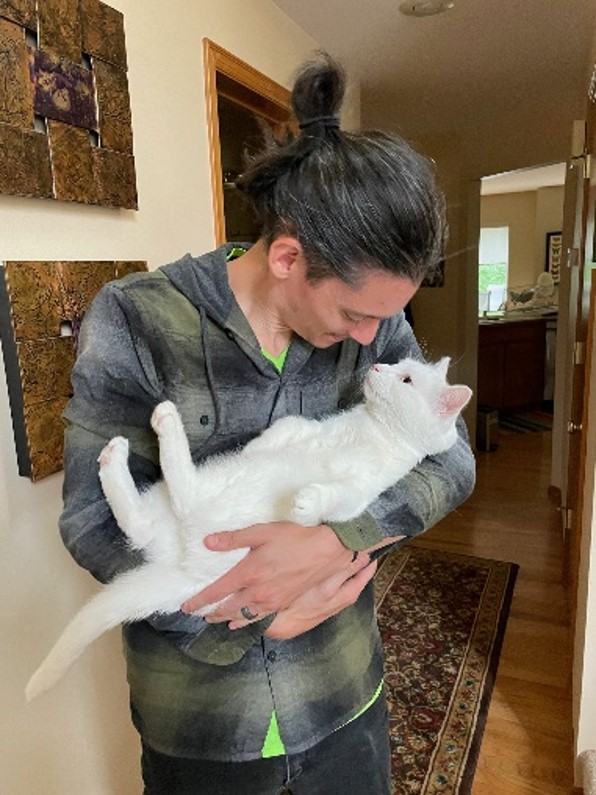
\includegraphics[width=\textwidth,height=2.08333in]{_img/GeoffMayhew.jpg}

\textbf{Geoff Mayhew, Data Analyst}\\
Research Fish Biologist (NMFS)\\
AFSC, Seattle

\textbf{Interests}

\begin{itemize}
\tightlist
\item
  professional: modeling, R coding, annual deployment planning\\
\item
  personal: travel, house projects, woodworking
\end{itemize}

\begin{center}\rule{0.5\linewidth}{0.5pt}\end{center}

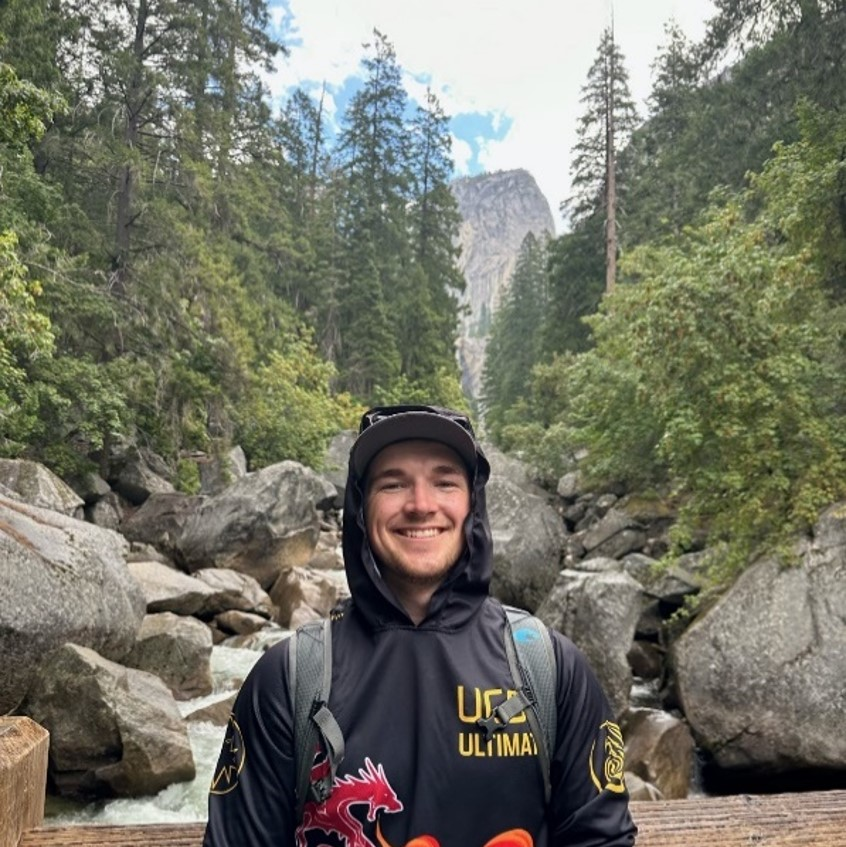
\includegraphics[width=\textwidth,height=2.08333in]{_img/CameronVanHorn.jpg}

\textbf{Cameron Van Horn, Data Analyst}\\
Pacific States Marine Fisheries Commission\\
AFSC, Seattle

\textbf{Interests}

\begin{itemize}
\tightlist
\item
  professional: data quality diagnostics and analytics\\
\item
  personal: film, music, photography, sports, snorkeling, diving
\end{itemize}

\begin{center}\rule{0.5\linewidth}{0.5pt}\end{center}

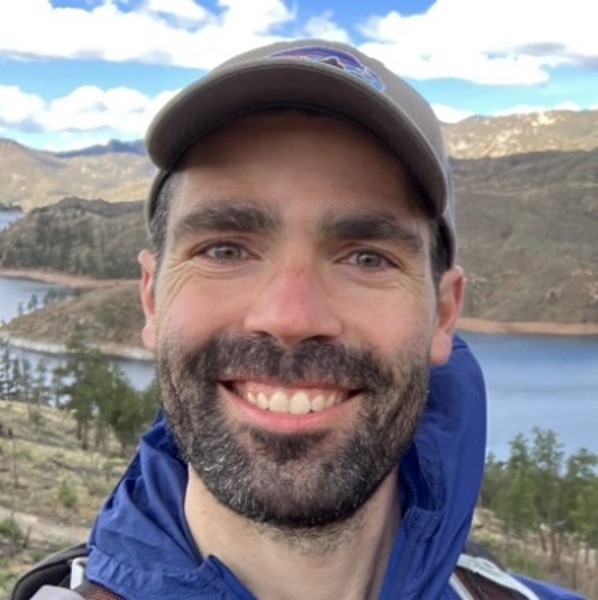
\includegraphics[width=\textwidth,height=2.08333in]{_img/PhilGanz.jpg}

\textbf{Phil Ganz, Data Analyst}\\
Fisheries Management Specialist (NMFS)\\
AKRO, Juneau

\textbf{Interests}

\begin{itemize}
\tightlist
\item
  professional: annual reporting, annual deployment planning, catch
  accounting, data quality\\
\item
  personal: family, running
\end{itemize}

You can learn more about Phil
\href{https://www.fisheries.noaa.gov/contact/phil-ganz}{here}

\begin{center}\rule{0.5\linewidth}{0.5pt}\end{center}

\section{How we meet}\label{how-we-meet}

\subsection{A-Team Meetings}\label{ateam-meetings}

\subsubsection{semimonthly Thursdays, 1000 PT, Google
Meet}\label{semimonthly-thursdays-1000-pt-google-meet}

Currently, as a whole team, we meet virtually by Google Meet every 2
weeks. We use Google Docs to set agendas, record decisions, and outline
action items during these meetings.

The
\href{https://docs.google.com/document/d/1WvOqt77kHU4_72IQFUuYN3M9kF2xTi56QtwpRFHf6C4/edit\#heading=h.32mfp9s1k5bh}{agenda}
is a single document -- this makes finding and referencing old agenda
items easier. At the end of each meeting, in prep for the next meeting,
the table and agenda outline are copied to the top of the page, the date
of the next meeting is added and any items or decisions that were
covered and settled or meetings that have passed are removed to make
space for the next meeting's items.

During the time between meetings, staff are expected to:

\begin{itemize}
\tightlist
\item
  fill in their updates in the table\\
\item
  review all the staff updates prior to the meeting and come with any
  questions\\
\item
  if appropriate, add items to the Discussion, Meetings or other
  sections of the agenda
\end{itemize}

\href{https://www.wordnik.com/words/scrivener}{Scrivener} duties for the
meeting rotate among A-Team staff and are listed at the bottom of the
agenda.

Scrivener Duties The Scrivener is responsible for:\\
1. Setting up the page for the next meeting (see above)\\
2. Running the meeting and keeping it on time\\
3. Documenting discussions and decisions, with help as needed from other
attendees

\subsection{1:1 with Jason}\label{meet-with-Jason}

Each team member has individual in-person meetings with Jason.\\
Each member is responsible for documenting their 1:1 meetings with
Jason, including tracking decisions and action items for themselves.
Jason is happy to collaborate in Google Docs with individuals if that is
their desire.

\section{How we give and receive
feedback}\label{how-we-give-and-receive-feedback}

Feedback, both giving and receiving it, is an important aspect of our
team. We expect feedback to be supportive but constructive. Feedback we
give and receive can come in a variety of places and times, including
but not limited to, during:

\begin{itemize}
\tightlist
\item
  brainstorming sessions\\
\item
  meetings\\
\item
  reviews of code or written documents\\
\item
  practice talks\\
\item
  post-project/post-meeting debriefs\\
\item
  1:1's
\end{itemize}

See the Feedback section of the \hyperref[code-of-conduct.qmd]{Code of
Conduct} for more discussion and some resources.

\section{How we share things}\label{how-we-share-things}

\textbf{Ask for help, and share what you learn and know:} Most of our
learning is done from each other. Struggling through problems alone is
inefficient. Ask for and give assistance with awareness of the value of
everyone's time.

We think it is useful to have standard ways of sharing things. These
don't always have to be followed but are a useful guide. The most
important principle is to make it easier for others and your future
self!

\begin{itemize}
\tightlist
\item
  Mechanisms for Sharing

  \begin{itemize}
  \tightlist
  \item
    Code: Github, Google Docs

    \begin{itemize}
    \tightlist
    \item
      GitHub account:
      \href{https://github.com/Alaska-Fisheries-Monitoring-Analytics}{Alaska
      Fisheries Monitoring Analytics}\\
    \end{itemize}
  \item
    Docs: Rmarkdown, Google Docs, or MSWord

    \begin{itemize}
    \tightlist
    \item
      \href{https://github.com/Alaska-Fisheries-Monitoring-Analytics/ateam-manual}{A-team
      Manual}\\
    \end{itemize}
  \item
    Network Drives

    \begin{itemize}
    \tightlist
    \item
      \texttt{Y://Programs\ Share/FMA\_Observers/Observer/A\ is\ for\ ANALYSIS/}\strut \\
    \item
      Google Drive: \texttt{FMA\ Analysis\ Group} (request access) \\
    \end{itemize}
  \item
    FMAnalytics G-Chat Space\\
  \item
    project specific G-Chat Spaces (e.g., SASH, ADP)\\
  \item
    Github Issues\\
  \end{itemize}
\item
  When sharing make sure to describe what you are sharing\\
\item
  A project-based approach to organizing your work makes it easier to
  share and solicit feedback from others

  \begin{itemize}
  \tightlist
  \item
    here is a
    \href{https://www.r-bloggers.com/2018/08/structuring-r-projects/}{good
    guide}\\
  \item
    see also \emph{Good enough practices in scientific computing}
    (Wilson et al. 2017))
  \end{itemize}
\end{itemize}

\begin{center}\rule{0.5\linewidth}{0.5pt}\end{center}

\bookmarksetup{startatroot}

\chapter[The Big Picture \{\#sec-big-picture\}]{\texorpdfstring{The Big
Picture
\{\#sec-big-picture\}\protect
\includegraphics[width=\textwidth,height=0.9375in]{_img/lightbulbicon.jpg}}{The Big Picture \{\#sec-big-picture\}}}\label{the-big-picture-sec-big-picture}

\href{https://www.youtube.com/watch?v=IlH0GgVbhwM}{Team culture} is a
set of values, goals and attitudes that members of the same team
practice to create a productive and healthy workplace atmosphere. It
represents all the ways people behave and the attitudes and beliefs that
inform those behaviors, including both the formal stated norms as well
as the implicit ways people interact.

The culture is
\href{https://www.youtube.com/watch?v=6MEocQzw-54}{everyone's
responsibility}.

\subsection{Benefits of a Strong
Culture}\label{benefits-of-a-strong-culture}

\begin{enumerate}
\def\labelenumi{\arabic{enumi}.}
\tightlist
\item
  A more enjoyable work environment\\
\item
  Greater engagement in the work\\
\item
  Conflict is managed in a healthy manner\\
\item
  Contributions are celebrated and valued\\
\item
  Inspires leadership - even among those who have no formal supervisory
  duties\\
\item
  Attracts and retains the best talent
\end{enumerate}

\href{https://www.youtube.com/watch?v=W5qQJhe7sLE}{Trust is the
foundation} for a strong culture.

\href{https://www.youtube.com/watch?v=jtpOYxsZj7o}{Hyper-competitiveness}
can be destructive to individuals and to a strong culture.

\section{Principles}\label{principles}

\section{NOTE: This section is still being developed with the help of
all Program
Staff.}\label{note-this-section-is-still-being-developed-with-the-help-of-all-program-staff.}

\subsubsection{Service}\label{service}

\href{https://www.noaa.gov/our-mission-and-vision}{NOAA's Mission}
statement is science, \textbf{service}, and stewardship. We are the
Analytical \textbf{Services} Program. Therefore, we should strive to
build a culture around service and adopt a service mindset by asking
``How can I help?''.

\textbf{Service} in practice\ldots{}\\
* puts the needs of others first\\
* actively listens\\
* asks questions\\
* suspends judgement\\
* is
\href{https://www.indeed.com/career-advice/career-development/how-to-be-empathetic}{empathetic}\\
* helps resolve issues and challenges\\
* exhibits
\href{https://www.indeed.com/career-advice/career-development/self-awareness-in-leadership}{self-awareness}\\
* shares time, knowlegdge, expertise, and energy

Even when the person being asked doesn't feel they need help,\\
\textbf{asking \texttt{How\ can\ I\ help?} has multiple benefits}
including:

\begin{enumerate}
\def\labelenumi{\arabic{enumi}.}
\tightlist
\item
  Making others feel supported\\
\item
  Reinforces the service mindset\\
\item
  Builds communication skills\\
\item
  Leads to broader opportunities for learning and growth\\
\item
  Produces better results\\
\item
  More positive about those you work with
\end{enumerate}

\subsubsection{Integrity}\label{integrity}

\subsubsection{Open-Mindedness}\label{open-mindedness}

\subsubsection{Personal Development}\label{personal-development}

\subsubsection{Science}\label{science}

\href{https://www.noaa.gov/our-mission-and-vision}{NOAA's Mission}
statement also includes \textbf{science}.

\section[Purpose - Why do we do
this?]{\texorpdfstring{\protect
\includegraphics[width=\textwidth,height=1.04167in]{_img/purpose_icon.png}Purpose
- Why do we do
this?}{Purpose - Why do we do this?}}\label{purpose---why-do-we-do-this}

We firmly believe that economically and environmentally sustainable
fisheries management:

\begin{itemize}
\tightlist
\item
  Must rely on data collected directly from commercial fishing vessels\\
\item
  The highest quality data is collected by scientific observers placed
  on commercial fishing vessels at sea or at shoreside processing
  plants\\
\item
  Both shoreside landing receipts and electronic monitoring do, and will
  continue to, play an important supporting role in providing data for
  fisheries management
\end{itemize}

We are committed to:

\begin{itemize}
\item
  Using all commercial fishing data sources, in combination with each
  other or other environmental or economic data when appropriate, to
  produce the best available science\\
\item
  Developing high-quality science for use in fisheries management and to
  advance the fields of fisheries science and management\\
\item
  Disseminating and communicating the best science based on these data\\
\item
  Sharing our data, knowledge, and advice to the greatest extent
  possible\\
\item
  Developing, enhancing, and fostering positive and strong
  collaborations among ourselves and our
  \hyperref[subsec-stakeholders]{stakeholders}
\item
  What is the inspiration that guides and motivates the team to achieve
  the mission?
\end{itemize}

\section[Mission - What do we
do?]{\texorpdfstring{\protect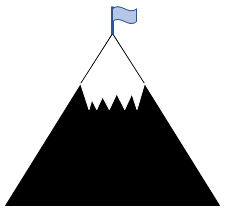
\includegraphics[width=\textwidth,height=0.52083in]{_img/mission_icon.png}Mission
- What do we
do?}{Mission - What do we do?}}\label{mission---what-do-we-do}

Our mission is to provide the highest quality best available science for
use in managing fisheries and marine resources.

The FMA Analytical Services Program adheres to NOAA's mission of
\href{https://www.noaa.gov/our-mission-and-vision}{Science, Service, and
Stewardship}.

Science\footnote{Scientific products might include (but is not limited
  to) data, data products, software, web applications, summaries,
  reports, analyses, models, presentations and advice.\\
} from the FMA A-Team:

\begin{itemize}
\tightlist
\item
  is rigorous, quantitative, and best available;
\item
  based on statistics and evidence and;
\item
  aims for transparency \& reproducibility.
\end{itemize}

Service from the FMA A-Team:

\begin{itemize}
\tightlist
\item
  is to provide the best-available science for use in decision-making;
\item
  based on clear, consistent and effective communication and
  collaboration;
\item
  aims to share data, knowledge, and information
\end{itemize}

Stewardship from the FMA A-Team:

\begin{itemize}
\tightlist
\item
  is to protect living marine resources, commercial fisheries, and the
  people who work in, on, or with marine ecosystems;
\item
  based on the diverse skill set and evolving abilities of the people
  and leveraged technologies and;
\item
  aims to be rational, ethical, and equitable.
\end{itemize}

What does the team aim to do to fulfill its purpose and achieve it's
vision?

\section{Internal Stakeholders}\label{subsec-stakeholders}

Internal stakeholders include:

\begin{itemize}
\tightlist
\item
  Each other (ASP staff)
\item
  FMA Staff\\
\item
  AFSC Staff\\
\item
  NOAA Staff
\end{itemize}

\section{External Stakeholders}\label{external-stakeholders}

External stakeholders often include, but are not limited to:

\begin{itemize}
\tightlist
\item
  \href{https://www.npfmc.org/}{NPFMC} and
  \href{https://www.npfmc.org/about-the-council/advisory-groups/}{advisory
  bodies}\\
\item
  Academics and other researchers\\
\item
  ADFG and other AK State personnel\\
\item
  NGO's\\
\item
  The U.S. Public
\end{itemize}

Alaska Native's and U.S. Federally recognized Tribal Nations are not
stakeholders. They are co-owners and co-managers of the resource. Find
out more
\href{https://www.noaa.gov/sites/default/files/2023-06/NOAA_Tribal_Consultation_Handbook\%202023_FINAL.pdf}{here}.

\bookmarksetup{startatroot}

\chapter{\texorpdfstring{Code of Conduct
\hspace{1cm}}{Code of Conduct }}\label{sec-code-of-conduct}

A \textbf{Code of Conduct} is a set of basic ground rules that we ask
team members to follow. The goal is to create an open and inclusive
space for our work that helps us achieve our collective goals. Along
with our \hyperref[sec-big_picture]{Big Picture}, the \textbf{Code of
Conduct}

\begin{itemize}
\tightlist
\item
  provides a benchmark for self-evaluation
\item
  helps define our identity
\item
  establishes behavioral guidelines
\end{itemize}

\textbf{We expect all team members to adhere to the policies and
guidelines outlined here, as well as those found in the
\href{https://drive.google.com/file/d/1wV0g2Tea0jdPjsTeNNST7I871j70qLAw/view}{AFSC
Code of Conduct}.}

\textbf{\emph{The FMA Analytical Services Program is dedicated to
providing a harassment-free experience for everyone, regardless of
gender, gender identity and expression, sexual orientation, disability,
physical appearance, body size, age, race, or religion. We do not
tolerate harassment of team members or others in our larger communities
in any form.}}

This code of conduct applies to all A-Team spaces, including group and
individual meetings (face to face and remote), workshops, email
correspondence, chat and web channels, and code repositories. Anyone who
violates this code of conduct may be sanctioned and referred to the
AFSC's policies.

\begin{center}\rule{0.5\linewidth}{0.5pt}\end{center}

\section{Managing Conflict}\label{managing-conflict}

To promote healthy resolutions to conflict, build trust, and develop a
sense of psychological safety on th A-Team, \textbf{all members of the
Analytical Services Program are expected to:}

\begin{enumerate}
\def\labelenumi{\arabic{enumi}.}
\item
  Delay entering into conversations when feelings are ``elevated''
  (i.e., high level of frustration, anger, upset, etc.)

  \begin{itemize}
  \tightlist
  \item
    Why? \href{https://www.youtube.com/watch?v=d_5DU5opOFk}{Anger
    impacts the way you process information}. Other emotions can have
    \href{https://nulab.com/learn/collaboration/overcoming-emotional-barriers-to-communication/}{negative
    impacts on communication} as well.\\
  \item
    What to do

    \begin{itemize}
    \tightlist
    \item
      If you are angry, do not confront the person until you are able to
      have a rational conversation where you are
      \href{https://welldoing.org/article/how-communicate-when-youre-angry}{open
      to hearing them and can actively listen}.\\
    \item
      If you are confronted by a person who is angry or upset

      \begin{itemize}
      \tightlist
      \item
        Do not to become defensive\\
      \item
        Politely request to delay the conversation\\
      \item
        Follow-up when emotions have settled
      \end{itemize}
    \end{itemize}
  \end{itemize}
\item
  Always
  \href{https://www.axios.com/2022/06/03/simple-workplace-principle-assume-positive-intent}{assume
  positive intent} of others. If your initial response is negative, try
  to change your viewpoint and find a positive explanation.
\item
  Recognize the humanity in yourself and others. This means:

  \begin{itemize}
  \tightlist
  \item
    Recognizing that no one is perfect, we all make mistakes.\\
  \item
    Gracefully and sincerely apologizing when mistakes are made.\\
  \item
    Gracefully accepting a sincere apology for mistakes when given.\\
  \item
    Cultivating real compassion for
    \href{https://youtu.be/-kfUE41-JFw}{yourself} and
    \href{https://www.youtube.com/watch?v=46bRW1pYgoY}{others}.
  \end{itemize}
\end{enumerate}

\href{https://www.youtube.com/watch?v=Lkj86o69c5c}{How to Actively
Listen}

\href{https://www.youtube.com/watch?v=RcGkHrPSzDc}{How to have an
uncomfortable conversation}

\begin{center}\rule{0.5\linewidth}{0.5pt}\end{center}

\section{Feedback}\label{feedback}

Feedback is meant to change outcomes. Feedback can be either
reinforcing, i.e., it reinforces behaviors or actions that lead to
outcomes we want, or redirecting, i.e., it outlines behaviors or actions
that lead to unwanted outcomes and provides alternative behaviors or
actions that lead to desired outcomes.

Giving and receiving redirecting feedback can be difficult. However, if
we don't get feedback, we can't see our own blind-spots. If we don't
provide constructive ways for others to improve, then we can't expect
them to improve and we can't expect to have our own needs met.

Healthy, productive teams have members who give each other six (6) or
more reinforcing feedback comments for every redirecting feedback
comment.

Reward your colleagues for good work and deeds.
\href{https://sites.google.com/noaa.gov/myafsc/home/workforce-collaboration-team-wct}{Here's
some ways to recognize them}.

Simon Sinek has some \href{https://youtu.be/tttv9lRPcLA?t=235}{great
advice} for how to give difficult feedback (watch at least to the 6:10
mark; but the whole clip is worthwhile).

Effective communication skills are like muscles, we need to exercise
them. You can't go to the gym for 9 hours and expect to be in shape. But
if you go for 30 minutes a day, every day, you will eventually get in
shape. Similarly, the first time you try to give or receive feedback in
a new way, it might go badly. But eventually it will get better and
easier - but never easy.

Not having a conversation because it will be hard is not an excuse for
not having a conversation. Difficult conversations avoided today become
tomorrow's even more difficult conversation.

This
\href{https://scwrl.ubc.ca/stem-writing-resources/learning-strategies-for-communicating-science/how-to-give-and-receive-effective-feedback/}{resource
from UBC} outlines best practices for giving and receiving feedback.

\href{https://www.youtube.com/watch?v=C0fRaM7M_WU}{How to Create a
Culture of Feedback}

\begin{center}\rule{0.5\linewidth}{0.5pt}\end{center}

\section{Psychological Safety}\label{psychological-safety}

\subsection{What is Psychological
Safety?}\label{what-is-psychological-safety}

All members of Analytical Services (including the Program Manager) are
expected to conform to a set of behavioral norms that are designed to
make the workplace a psychologically and physically safe space.

\begin{quote}
A \textbf{norm} is a rule that guides behavior toward the usual,
typical, and/or standard behavior of a group.
\end{quote}

A psychologically safe space is:

\begin{quote}
``a climate in which people are comfortable expressing and being
themselves.'' -- Amy Edmondson, \emph{The Fearless Organization}
\end{quote}

In practice, this means that people feel comfortable taking risks, being
themselves, speaking their minds, and being openly vulnerable in front
of co-workers. The ability to be vulnerable in a workplace is directly
related to the consequences that individuals feel they might be subject
to if they are openly vulnerable.

In a double-blind research study of teams,
\href{https://rework.withgoogle.com/guides/understanding-team-effectiveness/steps/introduction/}{Google}
found that the most important feature of highly effective teams was the
presence of
\href{https://rework.withgoogle.com/guides/understanding-team-effectiveness/steps/identify-dynamics-of-effective-teams/}{psychological
safety}.

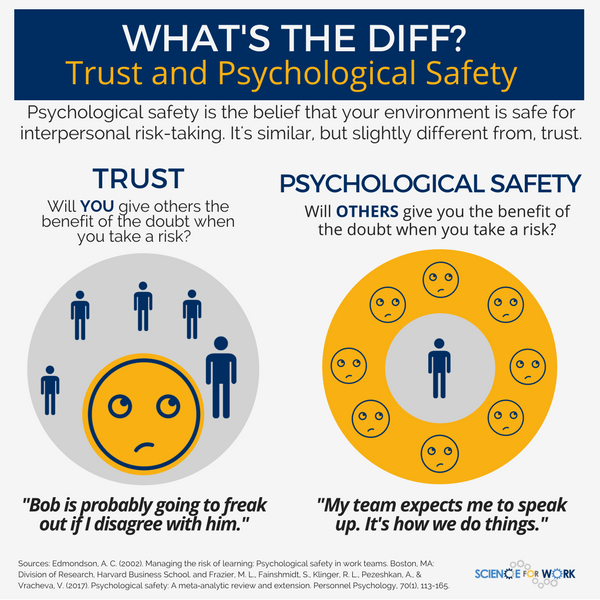
\includegraphics{_img/Trust_PsychSafety_Science4Work_icon.png}

\subsection{Why Do We Need Psychological Safety in the
Workplace?}\label{why-do-we-need-psychological-safety-in-the-workplace}

Evidence shows that creating a psychologically safe workplace is
strongly linked with highly effective teams\footnote{https://rework.withgoogle.com/guides/understanding-team-effectiveness/steps/identify-dynamics-of-effective-teams/}
which are more likely to share ideas, give and welcome feedback,
experiment, and discuss mistakes openly\textsuperscript{1,}\footnote{https://scienceforwork.com/blog/psychological-safety/}.
Psychologically safe workplaces are linked to higher employee
satisfaction\textsuperscript{2}

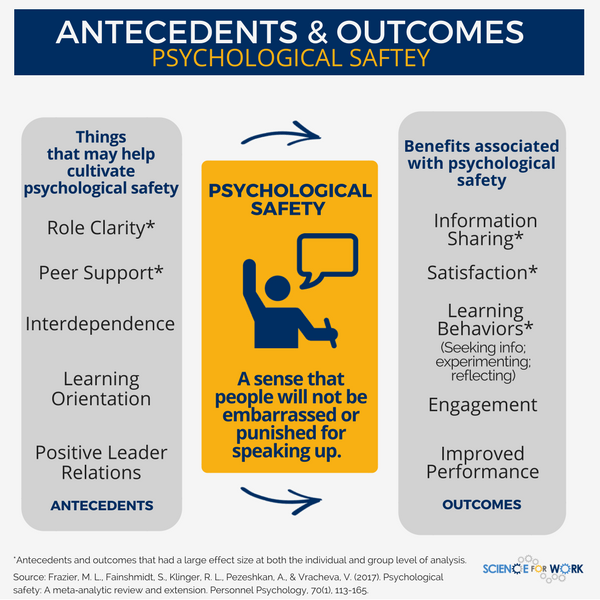
\includegraphics{_img/ANTECEDENTSOUTCOMES_PsychSafety_Science4Work_icon.png}

Both images above are from
\href{https://scienceforwork.com/blog/psychological-safety/}{Science for
Work}.

\subsection{How Do We Create Psychological Safety in the
Workplace?}\label{how-do-we-create-psychological-safety-in-the-workplace}

To promote psychological safety, we can:

\begin{enumerate}
\def\labelenumi{\arabic{enumi}.}
\tightlist
\item
  Develop self-awareness so that you can adjust your emotional responses
  and learn to react in a way that invites open discussion.\\
\item
  Demonstrate concern for other team members as people so that they feel
  comfortable speaking up and showing up as their whole selves.\\
\item
  Ask questions, show appreciation for other's ideas, and suspend
  judgement.\\
\item
  Engage in positive dialog to inspire honest conversations.\\
\item
  Own up to our mistakes and share learnings from failures.
\end{enumerate}

\begin{center}\rule{0.5\linewidth}{0.5pt}\end{center}

See also the resources for \hyperref[psych-safety]{Psychological Safety}
and \href{wellness-resources.qmd}{Wellness}

\begin{center}\rule{0.5\linewidth}{0.5pt}\end{center}

\section{Reporting Harassment}\label{reporting-harassment}

If you are being harassed by a member of the FMA A-Team, notice that
someone else is being harassed, or have any other concerns, please
contact the FMA Analytical Services Program Manager, Dr.~Jason Jannot,
at
\href{mailto:jason.jannot@noaa.gov}{\nolinkurl{jason.jannot@noaa.gov}}.
If you do not feel comfortable reporting to Jason, please contact
Jennifer Ferdinand (FMA Division Director) or Lisa Thompson (FMA Deputy
Director) or any other AFSC supervisor. Other methods of reporting
available to you include:

\begin{itemize}
\tightlist
\item
  \href{https://noaasashhelpline.org/}{NOAA Sexual Assault Sexual
  Harassment Helpline}
\item
  \href{https://www.noaa.gov/workplace-violence-prevention-response-program}{NOAA
  Workplace Violence Prevention and Response Program}
\item
  \href{mailto:DAO-955.OHCS@noaa.gov}{NOAA Workforce Management Office}
\item
  \href{mailto:noaa.oicr@noaa.gov}{NOAA Office of Inclusion and Civil
  Rights}
\end{itemize}

In addition to the AFSC's Code of Conduct, the Dec.~8th 2022
\href{https://www.noaa.gov/organization/inclusion-and-civil-rights/policy-statement-on-equal-employment-opportunity}{Policy
Statement on Equal Employment Opportunity} from NOAA provides a good
explanation of NOAA's stance and policies against harassment,
discrimination, and violence in the workplace.

\begin{center}\rule{0.5\linewidth}{0.5pt}\end{center}

\section{\texorpdfstring{\href{https://sites.google.com/noaa.gov/ohcs/employee-resources/work-life-resources/workplace-programs/drug-free-workplace-program}{Drug
Free Workplace}}{Drug Free Workplace}}\label{drug-free-workplace}

A drug-free workplace is a condition of employment for all federal
employees to refrain from using illegal drugs on or off-duty.

\bookmarksetup{startatroot}

\chapter{Onboarding}\label{sec-onboarding}

\section{Welcome to the FMA A-Team!}\label{welcome-to-the-fma-a-team}

Our group is excited that you have decided to join our team!

Here are some resources to help you get settled. We hope that these
on-boarding resources, guidelines, and tips will make your transition to
FMA seamless and enjoyable.

\href{https://drive.google.com/file/d/1Gxg-tw76NeptYFkya7M6JSyxsy31mmAu/view?usp=sharing}{AFSC
Onboarding Checklist for Federal and Non-Federal Staff}

For Federal FTEs, check out the following for many good resources:

\href{https://sites.google.com/noaa.gov/nmfs-erg-newhire/home?authuser=0}{NOAA
Fisheries New Hire Employee Resource Group}\\
\href{https://sites.google.com/noaa.gov/inside-fisheries-hc/human-capital/training-and-development/fisheries-onboarding-and-orientation-program}{Fisheries
New Employee Orientation website}\\
\href{https://drive.google.com/drive/folders/1aZcoJooHxNMh4kjCiv4WUgpDtszub1PI}{New
Employee Onboarding}

Foreign Nationals should review the
\href{https://sites.google.com/noaa.gov/myafsc/administrative/security/foreign-nationals}{AFSC
Interal Foreign Nationals webpage} during their first few days of
employment.

\section{CAC - Common Access Card}\label{cac---common-access-card}

A CAC will give you access to buildings and computer systems. It is the
necessary first step to getting started.

Both \textbf{Federal and non-Federal employees} will need a CAC.

Foreign Nationals (FN) \textbf{are not} assigned a CAC. FNs will need to
obtain a
\href{https://sites.google.com/noaa.gov/myafsc/technology/it-security/cac-waivers}{CAC
Waiver}. Work with your NOAA Sponsor.

\subsection{Get a New CAC}\label{get-a-new-cac}

CAC cards are only issued at Defense Department authorized locations
(referred to as ``RAPIDS'' offices) and may or may not be associated
with a NOAA facility. For AFSC staff, the following locations are the
closet RAPIDS stations.

\begin{enumerate}
\def\labelenumi{\arabic{enumi}.}
\item
  Seattle staff = WRC building 1, site ID 105831 (phone: 206-526-6571)
\item
  Juneau staff = Federal Bldg, site 102444 (phone: 907-463-2170)
\end{enumerate}

\subsection{Renew a CAC}\label{renew-a-cac}

See the
\href{https://sites.google.com/noaa.gov/myafsc/administrative/security/cac-renewal}{CAC
Renewal page} on MyAFSC.

\section{IT}\label{it}

On the first day, an A-Team member (likely Jason), will bring you to
OFIS to:

\begin{itemize}
\tightlist
\item
  get computer equipment
\item
  set-up accounts (including an Oracle database account)
\item
  get logged into NOAA computer \& Google account
\item
  \href{https://www.google.com/url?q=https\%3A\%2F\%2Fsites.google.com\%2Fnoaa.gov\%2Fmyafsc\%2Ftechnology\%2Fvpn-virtual-private-network&sa=D&sntz=1&usg=AOvVaw1YGm7HPymJCqrAYQakwJVj}{request
  a VPN account}
\item
  download software needed (e.g., R, RStudio, SQL Developer, Endnote)
\end{itemize}

\subsubsection{Confidential Data}\label{confidential-data}

Data used by the Analytical Services Program in it's raw\footnote{Raw
  here could mean the data has gone through QAQC processes as well as
  other processing. However, the data has \textbf{not} been summarized
  to meet the rule of three.} form is considered to contain confidential
information. As such, you will need to read and sign a Statement of
Non-Disclosure (SON). Work with the PM to get this completed in the
early days of on-boarding.

All confidential data must be summarized to meet the Rule of Three
before being shared with anyone who does not have a current, signed SON
on file with FMA. The rule of three requires that, when data is
aggregated, every data point in the aggregated data set includes a
minimum of three entities which mask the confidential information in
such a way that individual entities cannot be identified or tied to a
specific data point.

More general information on confidential data can be found
\href{https://sites.google.com/noaa.gov/myafsc/technology/it-security/privacy-impacts}{here}.

\subsubsection{Other IT Resouces}\label{other-it-resouces}

\href{https://sites.google.com/noaa.gov/myafsc/technology/onboarding-and-clearing-it}{IT
Onboarding webpage}\\
\href{https://sites.google.com/noaa.gov/myafsc/technology}{IT
Resources}\\
\href{https://sites.google.com/noaa.gov/myafsc/technology/afsc-it-service-desk}{IT
Help}\\
\href{https://sites.google.com/noaa.gov/myafsc/technology/it-security/software-management}{Software
Management and Permission}

\section{Schedules, Time \& Attendance}\label{schedules-time-attendance}

\subsubsection{non-Federal employees}\label{non-federal-employees}

Guidance on schedules, time and attendance should be provided by your
employer. Please also be sure to work with the A-Team Program Manager on
setting your schedule.

\subsubsection{Federal employees}\label{federal-employees}

If you are federal employee, you will access your time-sheets through
the \href{https://docwebta.eas.commerce.gov/webta/}{GovTA} web portal.
Within one week of on-boarding
\href{https://enterpriseservices.servicenowservices.com/es}{Enterprise
Services} will create a new profile for you in GovTA.

You should:

\begin{itemize}
\tightlist
\item
  work with the Program Manager to set your work schedule\\
\item
  familiarize yourself with the definitions and rules around
  \href{https://drive.google.com/file/d/1VlxkCEHZEdQd2pfGu9Bud5QZDUudqioa/view?pli=1}{Alternative
  Work Schedules}\\
\item
  fill out an
  \href{https://drive.google.com/file/d/1SvyTE2M6lQ0dcX5w3b0f7CJNxU6zDFDy/view?usp=share_link}{Employee
  Work Schedule Form}\\
\item
  fill out a
  \href{https://drive.google.com/file/d/19oABvmjMgRX4az-9U1Ijgd3ux5BwmHQw/view}{Telework
  Application Agreement}\\
\item
  fill out a
  \href{https://drive.google.com/file/d/198EkLWjTkQIOVQ1z7eD9eBf5z74Orfah/view}{Telework
  Safety Checklist}
\item
  fill out a
  \href{https://docs.google.com/forms/d/e/1FAIpQLSchGHo2aulpw4md1jFiEAnAtQ9NS-idmG9gJ_ngqlB-MQj3_w/viewform}{Telework
  Application Routing form}
\item
  take Telework Training in the
  \href{https://doc.csod.com/client/doc/default.aspx}{Common Learning
  Center}
\end{itemize}

\textbf{Telework Policy for NOAA FTEs - please note the following}

\begin{enumerate}
\def\labelenumi{\arabic{enumi}.}
\tightlist
\item
  You are currently (2024-07-01) required to be in the office 2 days per
  pay period.\\
\item
  Telework is a privilege which can be revoked.\\
\item
  If you are called into the office from telework status for any reason
  at any time during your normal teleworking hours, your commute to the
  office is \emph{non-work} time and should \emph{not} be recorded on
  your time sheet.

  \begin{itemize}
  \tightlist
  \item
    For example, your work computer becomes inoperable and AFSC Help
    Desk indicates that you need to bring it to the AFSC to have it
    fixed. Your travel time to the AFSC is not to be recorded as work
    time.
  \end{itemize}
\end{enumerate}

Forms and information can be found on the
\href{https://sites.google.com/noaa.gov/myafsc/administrative/time-and-attendance}{myAFSC
Time and Attendance page}

\href{https://sites.google.com/noaa.gov/myafsc/administrative/time-and-attendance}{Time
and Attendance Resources}

\subsection{Leave}\label{leave}

\subsubsection{non-Federal employees}\label{non-federal-employees-1}

Guidance on leave should be provided by your employer.

\subsubsection{Federal employees}\label{federal-employees-1}

Use GovTA to request leave. You can find resources related to leave
\href{https://sites.google.com/noaa.gov/myafsc/administrative/time-and-attendance}{here}

In 2023, NOAA added a new leave category
\texttt{66-Administrative\ Leave\ -\ Wellness}. The category
``\ldots aims to provide workplace liabilities that increase employees'
engagement, retention, and interest in their health and wellness.''
(\href{https://drive.google.com/file/d/1Z5XUCydpDjW-j8YLKRshp0WT_ZEfKKcq/view?pli=1}{HRGB
\#1018, FY23}). This program allows for up to 40 hours per year of leave
to participate in wellness activities during work hours. Below is some
guidance, but please see the
\href{https://drive.google.com/file/d/1Z5XUCydpDjW-j8YLKRshp0WT_ZEfKKcq/view?pli=1}{policy}
for a complete understanding of the rules and the
\href{https://drive.google.com/file/d/1asc745qKgQXn_7Tlp_DxnJhOYuYlROfX/view}{FAQ}
for further information.

Administrative Leave to participate in wellness activities:

\begin{enumerate}
\def\labelenumi{\arabic{enumi}.}
\tightlist
\item
  Must be coordinated with, requested to, and approved by your
  supervisor before being taken.\\
\item
  Must be displayed on your G-calendar.\\
\item
  Must be used in increments of at least 15 minutes.\\
\item
  Generally may not exceed more than 1 hour on any given work week.\\
\item
  May be used in conjunction with lunch periods, or at the beginning or
  end of a workday.\\
\item
  Must be used within the employee's established work hours.\\
\item
  Is not allowed on the employee's days off, or while the employee is
  otherwise on approved leave, or when the employee is on overtime.\\
\item
  May not be combined with other instances of approved Administrative
  Leave.
\end{enumerate}

See the
\href{https://drive.google.com/file/d/1Z5XUCydpDjW-j8YLKRshp0WT_ZEfKKcq/view?pli=1}{policy}
for eligibility, employee responsibilities and allowable activities.

\subsection{Working Over-Time (more than
40/80)}\label{working-over-time-more-than-4080}

\subsubsection{non-Federal employees}\label{non-federal-employees-2}

Obtain guidance on over-time from your employer.

\subsubsection{Federal employees}\label{federal-employees-2}

For Federal staff, there are three mechanisms for being compensated for
working more than 80 hours in a pay period (PP):

\begin{itemize}
\tightlist
\item
  Overtime Pay
\item
  Credit hours for those on maxi-flex schedules
\item
  Compensatory time
\end{itemize}

\paragraph{Overtime Pay}\label{overtime-pay}

Overtime pay is awarded for working beyond the 80 hours in a pay period.
This should not occur often during the year. As best as possible, please
work with the Program Manager ahead of time to gain approval for
overtime work. If you are on a Maxi-Flex schedule, Credit Hours can be
claimed \emph{in lieu} of overtime pay. Guidelines:

\begin{itemize}
\tightlist
\item
  Gain approval from Program Manager beforehand
\item
  Work with PM and Timekeeper to fill out paperwork
\end{itemize}

\paragraph{Credit Hours}\label{credit-hours}

If you are on a Maxi-Flex schedule, Credit Hours can be claimed \emph{in
lieu} of overtime pay. Guidelines:

\begin{itemize}
\tightlist
\item
  Can carry up to 24 credit hours\\
\item
  No advance approval is needed\\
\item
  Properly record credit hours on time-sheet\\
\item
  Submit a Request for Premium Pay in GovTA
\end{itemize}

\paragraph{Compensatory Time}\label{compensatory-time}

Compensatory time can be awarded for \textbf{travel} that occurs outside
or beyond normal working hours or days (e.g., ``red-eye'' flight, travel
on weekend, etc).

Compensatory time for working (as opposed to traveling) is typically not
awarded. Rather, overtime work is typically compensated via overtime pay
or credit hours (see above).

A quick guide for how to claim and record Compensatory Time for
traveling can be found
\href{https://docs.google.com/document/d/1BdvL0mbBE0JY5HkDjdoi5RhCc0rn3G0SfXFHeo03nzY/edit}{here}.

\section{Duties}\label{duties}

Both Federal and non-Federal employees will work with the PM to
determine specific responsibilities, individual projects, deliverables,
and duties. Duties and responsibilities will be revisited (with the PM,
and when appropriate, members of the A-Team) during the year and updated
to reflect any changes on a regular basis.

Duties that team members might assume, depending on interest, time,
Program/Division/Center priorities, and needs include (but are not
limited to):

\begin{itemize}
\tightlist
\item
  leading and assisting in designated research projects\\
  * Note that ``leading'' in this context means acting as Project
  Manager\\
\item
  participation in professional development opportunities
\item
  presenting analyses and results to NPFMC and other stakeholders\\
\item
  developing and submitting research funding proposals
\item
  submitting and publishing NOAA Technical Memorandum and other reports
\item
  submitting and publishing peer-reviewed journal articles
\item
  participating in outreach activities
\item
  attending scientific and professional conferences
\end{itemize}

\subsection{Observer Training Class}\label{observer-training-class}

The Program Manager \textbf{strongly encourages all new and existing
Program staff} to attend relevant portions of the 3 week observer
training class. This might be a requirement for any new staff members
who have never observed before or who have not had observer training
with FMA in the last 3 years.

More details can be found in the
\href{observer-training-classes.qmd}{Observer Training appendix}, but
check with the Program Manager or the FMA Training Program Manager for
the most up-to-date schedule.

\section{Performance}\label{sec-perf}

\subsubsection{non-Federal employees}\label{non-federal-employees-3}

Guidance on performance reviews should be provided by your employer.

\subsubsection{Federal employees}\label{federal-employees-3}

Soon after joining the A-Team, you should work with the PM to create an
annual, individual
\href{https://drive.google.com/file/d/18veCUTjncQVhRY6jOou9kclKWXJssOca/view?pli=1}{Performance
Plan}. Specific responsibilities, individual projects, deliverables, and
duties will be reflected in the individual Performance Plan. This
document will guide your work and will be revisited (in discussions with
the PM) during the year and updated to reflect any changes on an annual
basis.

Duties that team members might assume, depending on interest, time,
Program/Division/Center priorities, and needs are listed above under
\hyperref[duties]{Duties}.

More about the performance process can be found
\href{https://sites.google.com/noaa.gov/inside-fisheries-hc/human-capital/performance-culture-incentive-and-honorary-awards/commerce-alternative-personnel-system-caps}{here}.

The
\href{https://sites.google.com/noaa.gov/myafsc/administrative/workforce-management/awards}{AFSC
Awards page} lists the many ways Federal employees can be recognized and
awarded for their achievements including opportunities to nominate your
peers for their hard work.

\section{Facilities}\label{facilities}

AFSC buildings on the Seattle Sand Point Campus (a.k.a.
\href{https://www.wrc.noaa.gov/}{Western Regional Center {[}WRC{]}}) are
only accessible during work hours and with a CAC.

\href{https://www.wrc.noaa.gov/images/WRC_Map.jpg}{Map of NOAA Sand
Point Seattle Campus}

There is a cafeteria in Building 2 that offers snacks and drinks
(coffee, tea, etc.). Full lunch meals are no longer offered. As of
2024-07-01 WRC is experimenting with food trucks on campus on T,W, \&
Th, 1100-1330, located in the upper parking lot of Building 3.
Eventually there will be a Food Truck calendar.

\subsection{Office space}\label{office-space}

Our physical offices are in Building 4 of the WRC.\\
The following are FMA A-Team (and affiliated staff) office numbers:

\begin{itemize}
\tightlist
\item
  1060 -
  \href{https://www.fisheries.noaa.gov/contact/jason-e-jannot}{Jason
  Jannot, FMA Analytical Services Program Manager}
\item
  2060 - Cameron Van Horn, Data Management Specialist, PSMFC
\item
  1057 - Christian Gredzens, Research Fishery Biologist, NOAA
\item
  1057 - Andy Kingham, Operations Analyst, NOAA
\item
  1057 - Geoff Mayhew, Research Fishery Biologist, NOAA
\item
  1056 -
  \href{https://www.fisheries.noaa.gov/contact/craig-h-faunce}{Craig
  Faunce, Research Fisheries, NOAA Biologist}
\item
  1089 - Jennifer Cahalan, Statistician/Analyst, PSMFC
\end{itemize}

\textbf{Affiliated staff}

\begin{itemize}
\item
  Lacey Jeroue, AMMOP Program Manager, PSMFC\\
\item
  Alaska Regional Office (AKRO) Juneau A-Team collaborators

  \begin{itemize}
  \tightlist
  \item
    \href{https://www.fisheries.noaa.gov/contact/phil-ganz}{Phil Ganz}\\
  \item
    \href{https://www.fisheries.noaa.gov/contact/jason-gasper-phd}{Jason
    Gasper}\\
  \item
    \href{https://www.fisheries.noaa.gov/contact/jennifer-mondragon}{Jennifer
    Mondragon}
  \end{itemize}
\end{itemize}

Other FMA staff offices

\begin{itemize}
\tightlist
\item
  1059 -
  \href{https://www.fisheries.noaa.gov/contact/jennifer-ferdinand}{Jennifer
  Ferdinand, FMA Division Director}
\item
  1061 -
  \href{https://www.fisheries.noaa.gov/contact/lisa-thompson}{Lisa
  Thompson, FMA Deputy Director}
\item
  1062 -
  \href{https://www.fisheries.noaa.gov/contact/marlon-concepcion}{Marlon
  Conception, FMA Debriefing Program Manager}
\item
  1063 - \href{https://www.fisheries.noaa.gov/contact/brian-mason}{Brian
  Mason, FMA Training Program Manager}
\end{itemize}

\subsection{Reservations - Rooms \&
Vehicles}\label{reservations---rooms-vehicles}

Reservations for rooms or government vehicles can be found
\href{https://sites.google.com/noaa.gov/myafsc/reservations}{here}

\subsection{Parking}\label{parking}

To obtain either a vehicle or a bike parking pass for the Seattle Sand
Point Campus, contact Pass \& ID Security Office in Building 1
(206-526-6571). You will need to fill out a
\href{http://www.google.com/url?q=http\%3A\%2F\%2Fwww.wrc.noaa.gov\%2Fforms\%2FWRC\%2520Parking\%2520Decal\%2520v2008a.pdf&sa=D&sntz=1&usg=AOvVaw2YdnFqmKoV029T-pt6UwFj}{WRC
Parking Form}.

\subsection{Transit Benefits for
Bicyclists}\label{transit-benefits-for-bicyclists}

\subsubsection{Federal employees only}\label{federal-employees-only}

Allows for reimbursement to employees who use a non-motorized bicycle
for a substantial portion of travel between your residence and the work
site. Reimbursement can be up to \$20 per month, not to exceed \$240 per
calendar year for bicycle commuting expenses.

\href{https://sites.google.com/noaa.gov/cao/about-ocao/logistics-operations-division/noaa-transit-subsidy-program}{More
information on bike benefits and instructions}.

\subsection{Transportation Subsidy}\label{transportation-subsidy}

\subsubsection{Federal employees only}\label{federal-employees-only-1}

NOAA offers this non-taxable transit-fare subsidy program to encourage
federal employees to use public mass transportation while commuting to
and from work. Qualified employees are provided with a monthly benefit
based on the distance to and from work. The monthly maximum subsidy
transit benefit allowance is \$270. Unused benefits do not carry over to
the next month.

\href{https://sites.google.com/noaa.gov/cao/about-ocao/logistics-operations-division/noaa-transit-subsidy-program}{More
information on the transit subsidy program and application.}

\section{AFSC Contact Card}\label{afsc-contact-card}

Federal staff are encouraged to set-up an AFSC Contact Card, for
example, see
\href{https://www.fisheries.noaa.gov/contact/jason-e-jannot}{Jason's
Contact Card}. This is optional and not required but provides a public
facing profile so that others within and outside NOAA can find you and
can be linked to other social media accounts (e.g., Research Gate,
LinkedIn, etc.). You can request a
\href{https://docs.google.com/forms/d/e/1FAIpQLSdDfxoDycZjcmXDfPY_KnHwb2vPQ8HTzfFCSVt-qOvq_xPIZw/viewform}{Contact
Card here}

\section{Travel (Federal employees)}\label{travel-federal-employees}

To request domestic travel approval use the
\href{https://script.google.com/a/macros/noaa.gov/s/AKfycbwdQxgdDdWfoH_4bBK9xMfShQaqMPNogkTZx-VgC6tTx3aUMDogSxwEGWHWnAcZMSv4/exec}{Travel
App} for all domestic individual travel. For foreign travel requests,
please work directly with your travel arranger.

While on travel collect receipts for:\\
1. Lodging - ensure the balance shows 0.00 (zero)!\\
2. Local transport\\
3. Checked baggage charges

Receipts for food or other incidentals are not necessary.

Upon return:\\
1. Create and approve the final travel voucher in
\href{https://e2.gov.cwtsatotravel.com/}{E2}\\
2. Include receipts

\href{https://sites.google.com/noaa.gov/myafsc/administrative/travel}{AFSC
Travel FAQ}

\section{General Adminstrative
Resources}\label{general-adminstrative-resources}

\href{https://sites.google.com/noaa.gov/myafsc/administrative/general-admin}{General
Admin Resources}

\section{Health \& Safety}\label{health-safety}

Health and safety resources (e.g., reporting an accident) can be found
\href{https://sites.google.com/noaa.gov/myafsc/safety}{here}.

\bookmarksetup{startatroot}

\chapter[Expectations
\{\#sec-expectations\}]{\texorpdfstring{Expectations
\{\#sec-expectations\}\protect
\includegraphics[width=\textwidth,height=1.5625in]{_img/wearewilling.png}}{Expectations \{\#sec-expectations\}}}\label{expectations-sec-expectations}

\section{NOAA Fisheries CORE
Policies}\label{noaa-fisheries-core-policies}

Most of NOAA Fisheries policies can be found in the
\href{https://sites.google.com/noaa.gov/inside-fisheries-core/table-of-contents}{CORE
Policy Handbook}

Many other NOAA Fisheries employee resources can be found
\href{https://sites.google.com/noaa.gov/inside-fisheries/home}{here} .

\section{Professional Behavior}\label{professional-behavior}

All FMA Analytical Services staff (including the PM) are expected to
adhere to the code of conduct and norms of behavior listed in
\hyperref[sec-code-of-conduct]{Chapter 4 Code of Conduct} of this
manual.

It's important for all of us within the Program to \emph{always, always}
show respect and courtesy to others in all of our professional
communications and interactions -- that includes face-to-face, virtual
meetings, emails, phone calls, chat, and text. It also includes all
interactions among Program staff or any professional interactions
outside the Program.

\textbf{As a service Program our most important asset is our
relationships!}

Professional behavior includes, but is not limited to:

\begin{enumerate}
\def\labelenumi{\arabic{enumi}.}
\tightlist
\item
  Always using an appropriate tone and volume when speaking. Yelling is
  almost never necessary, unless there is an emergency or someone is in
  immediate danger.\\
\item
  Always using appropriate body language to help emphasize our point.
  When words and body language send different messages, humans defer to
  \emph{the message in the body language}. This means that intimidating
  body language such as leaning across a desk, getting into someone
  face, standing up, looming over a person, or beating our chest are all
  inappropriate behaviors in the workplace. They are counterproductive
  to getting your message across.\\
\item
  Always using appropriate language -- that means no swearing, no
  inappropriate or derogatory descriptions of others such as
  ``ignorant'', ``idiot'', ``stupid''. These create a toxic work
  environment and they are unnecessary and counterproductive.\\
\item
  Always work to support each other, not to undermine others. This means
  we do not ``talk trash'' or disparage others under any circumstances.
\end{enumerate}

See also the resources for \hyperref[psych-safety]{Psychological Safety}
and \href{wellness-resources.qmd}{Wellness}.

\section{Availability}\label{availability}

\begin{itemize}
\tightlist
\item
  Core hours for the AFSC are 9:30 am to 2:30 pm, T,W,Th.\\
\item
  A-Team members are encouraged to work in the office on one or more of
  these days.\\
\item
  Core hours do not apply on Monday or Friday.\\
\item
  NOAA Telework Policy for Federal employees requires 2 days in the
  office per pay period.\\
\item
  Non-Federal employees should follow the telework guidance from their
  employer.
\end{itemize}

You are \textbf{not} expected to be available 24/7. Similarly, unless it
is an emergency, do not expect responses to emails or any communication
before or after regular business hours on weekdays (6 am - 6 pm), or any
time on weekends/holidays/flex-days. However, because we recognize that
A-Team members should be able to create a working schedule that is right
for them, team members will not be penalized for sending communication
outside normal working hours.

\section{Google}\label{google}

\subsection{G-Mail}\label{g-mail}

We communicate largely via email on the A-Team. You should therefore
check your email at least once a day during the normal work week.

\subsection{G-Calendar}\label{g-calendar}

Much of our work is communicating and much of that communication comes
in the form of meetings. Therefore, you should:

\begin{itemize}
\tightlist
\item
  \hyperref[sec-calendar]{Make your calendar visible} to others.\\
\item
  Keep your calendar up-to-date\\
\item
  Add your working location and hours\\
\item
  Add leave and out of office (OOO) to your calendars\\
\item
  Set-up automated OOO message, if OOO for longer than 1 day\\
\item
  Busy/Private appointments during regularly scheduled work hours should
  only be used for non-work related activities for which there is
  approved leave, e.g., doctor's appointment, parental duties, etc.
  Please use ``Focus Time'' or other similar titles to block
  uninterrupted work time.
\end{itemize}

\section{Attendance at regularly scheduled
events}\label{attendance-at-regularly-scheduled-events}

Attendance, either virtual or in-person, is reasonably expected at:

\begin{itemize}
\tightlist
\item
  \hyperref[ateam-meetings]{Semimonthly A-Team meetings}
\item
  \hyperref[intro.qmdux5cux23meet-with-Jason]{Individual 1:1 with Jason}
  (in-person when possible)\\
\item
  Regularly scheduled project meetings\\
\item
  \href{https://www.npfmc.org/current-or-next-council-meeting/}{NPFM
  Council Meetings}\\
\item
  FMA All-hands
\end{itemize}

Attendance is strongly recommended when possible at:

\begin{itemize}
\tightlist
\item
  AFSC All-Hands\\
\item
  Other Center-wide Meetings
\end{itemize}

\subsection{Tardiness \& Absence}\label{tardiness-absence}

Let's face it - life happens. Be kind. If you're going to be late,
please notify someone else in the meeting as soon as you realize it and
provide a time frame for arrival. If you know in advance that you aren't
going to attedn the meeting, decline on your calendar.

\section{Expectations of the Program
Manager}\label{expectations-of-the-program-manager}

As of 2024, Jason Jannot is the FMA Analytical Program Manager. You can
read about his \hyperref[sec-jj-philosophy]{leadership and management
philosophy here}.

The Program Manager will (at a minimum) provide the A-Team with:

\begin{itemize}
\tightlist
\item
  Clarity (the \texttt{why?})\\
\item
  Guidance (the \texttt{how?})\\
\item
  Expectations (the \texttt{what?})\\
\item
  Collaboration \& Communication (the \texttt{who?})\\
\item
  Prioritization \& Gate-keeping\\
\item
  Accountability\\
\item
  Visibility \& Public Recognition\\
\item
  Support Overcoming Barriers\\
\item
  Timely Administrative Support\\
\item
  A Professional and Ethical Role Model
\end{itemize}

In addition to the above, the Program Manager will (at a minimum)
provide individual team members with:

\begin{itemize}
\tightlist
\item
  Positive feedback \& constructive criticism on work\\
\item
  Professional career support and development, including but not limited
  to:

  \begin{itemize}
  \tightlist
  \item
    opportunities for

    \begin{itemize}
    \tightlist
    \item
      training\\
    \item
      presenting (e.g., conferences, meetings, outreach, etc.)\\
    \item
      publishing
    \item
      advancing (e.g., promotion, details, etc.)\\
    \item
      collaborating\\
    \item
      leading\\
    \item
      mentoring
    \end{itemize}
  \end{itemize}
\item
  Regular meetings to discuss work \& maintain progress on goals\\
\item
  Empathetic listening\\
\item
  Coaching
\end{itemize}

\section{Expectations of Team
Members}\label{expectations-of-team-members}

A-Team members will (at minimum):

\begin{itemize}
\tightlist
\item
  behave professionally and ethically in all work interactions
\item
  strive to produce the best science, given the constraints\\
\item
  grow and maintain technical and inter-personal skills
\item
  share knowledge, experience, code, and time\\
\item
  adopt a \href{https://www.youtube.com/watch?v=q0mzqUMAc20}{service
  mindset}
\item
  adopt a
  \href{https://www.youtube.com/watch?v=AMG8ObDmbaM}{collaborative
  working mindset}\\
\item
  adapt and be flexible, within reason\\
\item
  communicate clearly and effectively
\item
  communicate both successes and sticking points regularly\\
\item
  contribute to creating a positive, inclusive, and safe work culture
\end{itemize}

Remember, as a government agency, we serve the people of the United
States and \emph{service} is 1/3\textsuperscript{rd} of
\href{https://www.noaa.gov/our-mission-and-vision}{NOAA's mission}.
Adopting a service mindset when approaching each other, stakeholders,
partners, and collaborators will magnify our positive impacts on marine
ecosystems, commercial fishing, and the wider world.

Some ways to adopt a service mindset:

\begin{itemize}
\tightlist
\item
  Share - \href{collaborate.qmd}{code}, knowledge, resources,
  opportunities
\item
  Serve as a role model\\
\item
  Serve as a resource for other members of the A-Team\\
\item
  Nominate your peers for their hard work and achievements -
  \href{https://sites.google.com/noaa.gov/myafsc/administrative/workforce-management/awards}{AFSC
  Awards page}.
\item
  Participate in outreach activities
\item
  Mentor others when appropriate, especially new team members
\end{itemize}

\section{Team Collaboration and
Communication}\label{team-collaboration-and-communication}

Although the Program Manager is your primary supervisor, everyone should
always feel like they can reach out to anyone else on the A-team for
help or collaboration.

\begin{center}\rule{0.5\linewidth}{0.5pt}\end{center}

``We are Willing to Try'' artwork © Samantha Tustison Snyder, Doodle Art
Alley Inc.

\bookmarksetup{startatroot}

\chapter[Communication
\{\#communication\}]{\texorpdfstring{Communication
\{\#communication\}\protect
\includegraphics[width=\textwidth,height=0.72917in]{_img/communication_icon.png}}{Communication \{\#communication\}}}\label{communication-communication}

There is a plethora of communication methods and technologies. However,
the communication tool should be chosen based on the purpose of the
communication. The purpose of this section is to explain how
communication tools differ so that the tool used is appropriate given
the topic(s) and timelines.

\section[Email ]{\texorpdfstring{Email
\protect
\includegraphics[width=\textwidth,height=0.3125in]{_img/email_icon.png}}{Email }}\label{email}

\textbf{Topics}: Single topics requiring simple or little or no context,
explanation, or discussion\\
\textbf{Time}:

\begin{itemize}
\tightlist
\item
  Immediate action is not required and/or;\\
\item
  Discussion is very limited or unnecessary and/or;\\
\item
  Completion time is not pressing
\end{itemize}

\textbf{Tone}: It can be very difficult to get the right tone in an
email. Sometimes it's worthwhile to write the email but delay sending
it. Then go back and check the tone after taking a pause.\\
\textbf{Pros}: Creates a record\\
\textbf{Cons}: Can be slow, lost, ignored\\
\textbf{Tracking}: Formally captured in writing - creates a record\\
\textbf{Uses}:

\begin{itemize}
\tightlist
\item
  Simple requests for a single action or, at most, a few closely related
  actions\\
\item
  Short summary of a single topic\\
\item
  Routine tasking\\
\item
  Follow-up summaries from video calls/FTF/phone calls
\end{itemize}

\textbf{Consider}: moving to a video call/FTF or phone call if the email
chain goes back and forth more than a few times or in-depth discussion
is necessary.

\section[Video call/Face-To-Face Meeting (FTF) ]{\texorpdfstring{Video
call/Face-To-Face Meeting (FTF)
\protect
\includegraphics[width=\textwidth,height=0.3125in]{_img/FTF_Vchat_icon.png}}{Video call/Face-To-Face Meeting (FTF) }}\label{video-callface-to-face-meeting-ftf}

You are expected to follow the
\href{https://docs.google.com/document/d/1K8mBHH6JOdKC4aT0L4jHmTJot9n4fnW9_L9kwdclCkQ/edit\#heading=h.wwlwg0rdx3c8}{AFSC
Guidance on Inclusive Meetings in Hybrid Work Environments}. The
\href{https://docs.google.com/presentation/d/1D9cA_HwDdASXM5VfEV4l6n8_h7GG4ieXiAD4a9Lo0jo/edit\#slide=id.p}{slide
deck} from the AFSC FAQ session describing this guidance is also
available.

\textbf{Topics}: Sensitive, complex, or multiple topics\\
\textbf{Time}: Lengthy discussion necessary; actions or responses will
be discussed\\
\textbf{Tone}: Voice inflection, body language and body posture can be
distorted or hidden by the tech. Eye contact can be misinterpreted,
misleading, or absent.\\
\textbf{Pros}: Can screen share/show\\
\textbf{Cons}: Requires some planning\\
\textbf{Tracking}: No formal tracking - requires participants to take
notes; Video calls can be recorded.\\
\textbf{Use}:

\begin{itemize}
\tightlist
\item
  To collaborate with team members\\
\item
  To build rapport and relationships\\
\item
  To provide or receive feedback\\
\item
  To provide or receive coaching\\
\item
  For instructional/side-by-side training/teaching\\
\item
  When there are multiple participants\\
\item
  When screen sharing/showing is needed
\end{itemize}

\textbf{Consider}: using other methods for simple updates that are
informational only and require no response.

\section{Chat}\label{chat}

\textbf{Topics}: Single, non-sensitive topics which require no
explanation, sharing general information (e.g., links, papers, etc.)\\
\textbf{Time}:

\begin{itemize}
\tightlist
\item
  Immediate response is necessary, requested or implied
\item
  Discussion is very limited or unnecessary
\item
  Very simple responses expected
\end{itemize}

\textbf{Tone}: Fast pace can lead to misunderstandings of tone and
intent, similar to email.\\
\textbf{Pros}: Fast\\
\textbf{Cons}:

\begin{itemize}
\tightlist
\item
  No record created\\
\item
  Limited ability to engage in depth\\
\item
  Links to files will be lost if history is turned off
\end{itemize}

\textbf{Tracking}: No formal tracking - requires participants to take
notes or screen shots.\\
\textbf{Use}:

\begin{itemize}
\tightlist
\item
  To ask simple questions\\
\item
  To check-in for current/near-future availability\\
\item
  Share informational link\\
\item
  Real-time discussion among team during formal meetings, e.g., FMAC,
  PCFMAC, Council, etc. - though discussion will be limited
\end{itemize}

\textbf{Consider}: moving lengthy discussions to a video call or FTF.

\section[Phone ]{\texorpdfstring{Phone
\protect
\includegraphics[width=\textwidth,height=0.3125in]{_img/phone_icon.png}}{Phone }}\label{phone}

\textbf{Topics}: Sensitive or complex topics\\
\textbf{Time}:

\begin{itemize}
\tightlist
\item
  Immediate response or action is necessary\\
\item
  Discussion could be lengthy\\
\item
  Completion time is pressing
\end{itemize}

\textbf{Tone}: Voice inflection can be distorted, lost or misinterpreted
due to tech; requires careful listening and voice control.\\
\textbf{Pros}: Can address time sensitive issues quickly\\
\textbf{Cons}: No screen show/share, body language missing\\
\textbf{Tracking}: No formal tracking - requires participants to take
notes\\
\textbf{Use}:

\begin{itemize}
\tightlist
\item
  Emergencies\\
\item
  Urgent, time sensitive requests\\
\item
  Contact necessary during off-hours or off-days\\
\item
  When video call/FTF is not possible but topics are sensitive or
  complex\\
\item
  Quick topics that are time sensitive
\end{itemize}

\textbf{Consider}: following up with an email summary of the
conversation

\section[Mobile Text/SMS ]{\texorpdfstring{Mobile Text/SMS
\protect
\includegraphics[width=\textwidth,height=0.41667in]{_img/communication_icon.png}}{Mobile Text/SMS }}\label{mobile-textsms}

\textbf{Topics}: Extremely time sensitive topics or contact necessary
outside normal work days/hours, requires zero explanation\\
\textbf{Time}:

\begin{itemize}
\tightlist
\item
  Immediate response or action is necessary
\item
  No discussion
\item
  Very simple responses expected
\end{itemize}

\textbf{Tone}: Fast pace can lead to misunderstandings of tone and
intent, similar to email and chat.\\
\textbf{Pros}: Can address time sensitive issues quickly\\
\textbf{Cons}: No screen show/share\\
\textbf{Tracking}: Creates a record, but there might be limits and
constraints\\
\textbf{Use}:

\begin{itemize}
\tightlist
\item
  Emergencies\\
\item
  Urgent, time sensitive requests\\
\item
  Necessary contact during off-hours or off-days\\
\item
  To check-in for current/near-future availability
\end{itemize}

\textbf{Consider}: moving to another method as soon as practicable.

\bookmarksetup{startatroot}

\chapter{Collaboration \& Code Review}\label{collaborate.qmd}

\section{NOTE: These sections will be completed with input from all
Analytical Services Program members during the Analytical Services
Program Launch Meeting slated for early
2024.}\label{note-these-sections-will-be-completed-with-input-from-all-analytical-services-program-members-during-the-analytical-services-program-launch-meeting-slated-for-early-2024.}

\section{Git Manager Software}\label{git-manager-software}

Here are some apps (called
``\href{https://en.wikipedia.org/wiki/Client_(computing)}{clients}'')
you can use to help you manage your Git interface (i.e., less command
line, more point-and-click):

\href{https://git-fork.com/}{Fork} - Jason's favorite and it's free and
easy to install\\
\href{https://geo.uzh.ch/microsite/reproducible_research/post/rr-rstudio-git/}{Rstudio}
- has a built-in Git interface\\
\href{https://desktop.github.com/}{GitHub Desktop} - probably one of the
more famous clients\\
\href{https://www.sourcetreeapp.com/}{sourcetree} - another common one

You can read about those and many others
\href{https://blog.devart.com/best-git-gui-clients-for-windows.html\#GitHub-Desktop}{here}.

\section{NOAA Open Science Git
Resources}\label{noaa-open-science-git-resources}

\href{https://nmfs-opensci.github.io/GitHub-Guide/\#sec-introduction}{GitHub
and Git NOAA Open Scapes resources}

\section{Collaboration using Git}\label{collaboration-using-git}

Currently, this is an amalgamation of
\href{https://docs.google.com/document/d/1lcchh6ggKS5-Sf7G3zwyRz1AA_XVxb7rc8Id_k5GEOo/edit\#heading=h.k1i0lpeyjkx}{Jason's
Git Collaboration notes} and the
\href{https://docs.google.com/document/d/1spu2uv0KmV2_aW64qwe2pJndPrSeHNEj1Utzi_lLpjU/edit\#heading=h.84v7rojjdy4y}{2024
ADP Team Charter}

Determining the
\href{https://www.atlassian.com/git/tutorials/comparing-workflows}{``Git
Work Flow''} is a huge part of working in a team! Be sure to check out
the ``Guidelines'' section in the previous link for best practices when
developing a workflow.


\includegraphics[width=\textwidth,height=2.08333in]{_img/git.png}

\begin{quote}
Jason suggests the Centralized Workflow (see link above) which keeps a
linear history\footnote{If you don't like the Centralized Workflow, try
  the
  \href{https://www.atlassian.com/continuous-delivery/continuous-integration/trunk-based-development}{Trunk-based
  Workflow}.}.
\end{quote}

\subsubsection{How to Collaborate}\label{how-to-collaborate}

\begin{enumerate}
\def\labelenumi{\arabic{enumi}.}
\tightlist
\item
  Add collaborators to repository\\
\item
  Collaborators clone repository to their local machine\\
\item
  Make changes

  \begin{enumerate}
  \def\labelenumii{\alph{enumii}.}
  \tightlist
  \item
    Create a New Branch\\
  \item
    Name it appropriately e.g., jason/newfeature\\
  \item
    Make changes locally on the new branch\\
  \item
    Commit changes to the new branch

    \begin{enumerate}
    \def\labelenumiii{\roman{enumiii}.}
    \tightlist
    \item
      As a general rule, you should commit when you finish something
      that allows your code to work - usually ends up being a couple
      times an hour.\\
    \end{enumerate}
  \item
    \emph{See below before completing this step} - Push changes to the
    remote repository\ldots this will create a pull request\ldots.
  \end{enumerate}
\end{enumerate}

\subsubsection{Before Pushing to the
Repository}\label{before-pushing-to-the-repository}

\begin{enumerate}
\def\labelenumi{\arabic{enumi}.}
\tightlist
\item
  Switch to your local main branch (\texttt{\$git\ checkout\ main})\\
\item
  Pull the remote main into your local main
  (\texttt{\$git\ pull\ origin\ main})\\
\item
  Switch to your dev branch
  (\texttt{\$git\ checkout\ \textless{}your-dev-branch-name-here\textgreater{}})\\
\item
  Merge your local main to your local dev branch
  (\texttt{\$git\ merge\ main})

  \begin{enumerate}
  \def\labelenumii{\alph{enumii}.}
  \tightlist
  \item
    \textbf{NOTE} This is where conflicts will show up if they will
    occur\\
  \item
    Fix any conflicts
  \end{enumerate}
\item
  Do some checking before pushing:

  \begin{enumerate}
  \def\labelenumii{\alph{enumii}.}
  \tightlist
  \item
    Check the commits that will be pushed
    (\texttt{\$git\ log\ -\ -\ oneline}; \texttt{q} escapes you back to
    the \texttt{\$})\\
  \item
    Check your connection (\texttt{\$git\ remote\ -v})\\
  \end{enumerate}
\item
  Push your changes
  (\texttt{\$git\ push\ origin\ \textless{}your-branch-name\textgreater{}})
\end{enumerate}

\section{Code Review}\label{code-review}

\subsection{Pull Request}\label{pull-request}

A pull request is a request by a collaborator for the repo owner to
``pull'' the new code into the main branch (or other branch) which will
then reflect those changes on the remote repos when others pull that
branch down.

\paragraph{Pull Request - What are they good
for?}\label{pull-request---what-are-they-good-for}

Pull request can simplify code review. They are a discussion point
between coders. They can be used to:

\begin{itemize}
\tightlist
\item
  review and discuss code: a new feature, improvements, strategy, etc.
\item
  address issues
\item
  any time new code is added to the repo
\end{itemize}

\textbf{What are the benefits of pull requests as code
review\footnote{For a counter argument to pull requests,
  \href{https://youtu.be/ASOSEiJCyEM?t=275}{see this video}}?}

\begin{enumerate}
\def\labelenumi{\arabic{enumi}.}
\tightlist
\item
  Increases the quality of the code
\item
  Decreases probability of breaking stuff
\item
  Frees time from micromanaging other peoples code
\item
  Reduces the need for meetings
\item
  Email notifications act as the interface
\item
  They create a history - all discussion \& code (even if it is
  ultimately rejected), lives on a branch
\end{enumerate}

The downsides include (see also\textsuperscript{2}):\\
1. You have to wait to have your code reviewed by others\\
2. Reviewer can get backed up \& overwhelmed

\paragraph{How to Submit a Pull
Request}\label{how-to-submit-a-pull-request}

\begin{enumerate}
\def\labelenumi{\arabic{enumi}.}
\tightlist
\item
  Go to the repo, at the top click on \texttt{Pull\ Requests}\\
\item
  Create a \texttt{New\ Pull\ Request} (green button upper right)\\
\item
  Ensure you are comparing the right branches\\
\item
  Look at the \texttt{gitdiff}\\
\item
  Give it an appropriate succinct title\\
\item
  Include a descriptive message

  \begin{enumerate}
  \def\labelenumii{\alph{enumii}.}
  \tightlist
  \item
    What has been done\\
  \item
    How to use the new code\\
  \item
    What someone could do to test the code, e.g., do\ldots{}\\
  \end{enumerate}
\item
  Create the request\\
\item
  Add a reviewer - upper right hand corner. Will trigger an email.\\
\item
  Once reviewed, the pull request will be merged with the branch
  (typically main)
\end{enumerate}

NOTE: You can add more commits to a single pull request, provided it has
not been reviewed and merged. \emph{However}, only do this for very
minor changes - missing spaces, typos, missing last lines etc.

\paragraph{How to Review a Pull
Request}\label{how-to-review-a-pull-request}

\begin{enumerate}
\def\labelenumi{\arabic{enumi}.}
\tightlist
\item
  Open the pull request\\
\item
  Review the code changes\\
\item
  Reviewer - provide comments and feedback as comments\\
\item
  Originator - respond to comments, perhaps add comments\\
\item
  Reviewer - Approve changes (upper right corner) and add approval
  comment\\
\item
  Reviewer - merge pull request\\
\item
  Originator - delete the branch once the code has been merged.
  \emph{Please do this so that our remote is clean!}\\
\item
  \emph{DONT FORGET TO PULL} the new code to your local instance to get
  latest code.
\end{enumerate}

\section{Issues}\label{issues}

Issues are a great way to improve code outside the normal pull
request-review process. Issues can be used to propose:

\begin{enumerate}
\def\labelenumi{\arabic{enumi}.}
\tightlist
\item
  Fixes to broken code\\
\item
  Cool new features\\
\item
  Tackle TODO lists\\
\item
  Document Q\&A
\end{enumerate}

Use \texttt{tags} (right sidebar) to highlight the type of issue being
submitted.

\subsection{How to submit an Issue}\label{how-to-submit-an-issue}

\begin{enumerate}
\def\labelenumi{\arabic{enumi}.}
\tightlist
\item
  Open an issue\\
\item
  Give it a succinct but appropriate name\\
\item
  Give it a \texttt{tag}\\
\item
  Use the \texttt{@} in the body of the issue to mention others who
  might be interested or involved in the issue resolution\\
\item
  Use simple pseudo-code (via Markup code) to describe your proposed
  changes.\\
\item
  Provide a minimal reproducible example for bugs/errors, a.k.a. a
  \href{https://stackoverflow.com/help/minimal-reproducible-example}{repex}\\
\item
  Be sure to close the issue once it is complete.

  \begin{enumerate}
  \def\labelenumii{\alph{enumii}.}
  \tightlist
  \item
    Pro Tip: You can use the following statement to make Github
    automatically close an issue:\\
    \texttt{this\ closes\ issue\ \#\textless{}insert-issue-num\textgreater{}}
    \href{https://github.com/jjannot-NOAA/PlantSamplingAnalysis/issues/5\#issuecomment-1480164759}{see
    example here}
  \end{enumerate}
\end{enumerate}

\subsection{Assigning Issues}\label{assigning-issues}

\begin{enumerate}
\def\labelenumi{\arabic{enumi}.}
\tightlist
\item
  Feel free to assign yourself the issue, but be sure to eventually
  tackle the issue.
\item
  \emph{BEFORE ASSIGNING TO OTHERS} discuss with the other person and/or
  the PM to ensure assignment is appropriate and does not conflict with
  current priorities.
\end{enumerate}

\section{Compare Two Branches on
GitHub}\label{compare-two-branches-on-github}

\begin{enumerate}
\def\labelenumi{\arabic{enumi}.}
\tightlist
\item
  Open the branch with the newest commits
\item
  At the top you'll see the number of commits difference like this:
\end{enumerate}

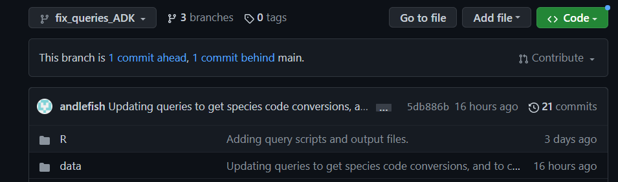
\includegraphics{_img/github_compare_2_branches.png}

\begin{enumerate}
\def\labelenumi{\arabic{enumi}.}
\setcounter{enumi}{2}
\tightlist
\item
  Click on the link ``\textless\#\textgreater{} commit ahead''
\item
  That will bring you to the diff page! Voila!
\end{enumerate}

\section{To link a pull request with an
issue}\label{to-link-a-pull-request-with-an-issue}

\href{https://docs.github.com/en/issues/tracking-your-work-with-issues/linking-a-pull-request-to-an-issue}{Link
Pull Request with Issue}

See \href{more-git.qmd}{Git Tips} for additional tips and resources.

\bookmarksetup{startatroot}

\chapter[Publications by FMA Analytical Services
\{\#sec-publications\}]{\texorpdfstring{Publications by FMA Analytical
Services
\{\#sec-publications\}\protect
\includegraphics[width=\textwidth,height=0.72917in]{_img/journalarticleicon.png}}{Publications by FMA Analytical Services \{\#sec-publications\}}}\label{publications-by-fma-analytical-services-sec-publications}

\section{Peer-Reviewed Publications}\label{peer-reviewed-publications}

\subsection{2024}\label{section}

\subsection{2023}\label{section-1}

\begin{itemize}
\item
  Cheng, M L H, C. J. Rodgveller, J. A. Langan, C. J Cunningham. 2023.
  \href{https://doi.org/10.1093/icesjms/fsad037}{Standardizing
  fishery-dependent catch-rate information across gears and data
  collection programs for Alaska sablefish (\emph{Anoplopoma fimbria}).
  ICES J. Mar.~Sci. 80(4):1028 - 1042}.
\item
  Faunce, C., J. Smith, A. Kingham, D. Jaszka. 2023.
  \href{https://doi.org/10.1016/j.marpol.2023.105868}{Fisheries
  observers as enforcement assets: 21 Years of lessons from the North
  Pacific. Marine Policy 158: 1-12}. See also
  \href{https://www.fisheries.noaa.gov/feature-story/advancing-transparency-fisheries-monitoring-and-enforcement}{WebStory}
\end{itemize}

\begin{center}\rule{0.5\linewidth}{0.5pt}\end{center}

\section{Technical Memoranda and Other
Reports}\label{technical-memoranda-and-other-reports}

\subsection{2024}\label{section-2}

\begin{itemize}
\item
  \href{https://www.fisheries.noaa.gov/s3//2023-11/Final-2024-ADP.pdf}{2024
  Annual Deployment Plan for Observers and Electronic Monitoring in the
  Groundfish and Halibut Fisheries off Alaska}
\item
  \href{https://www.fisheries.noaa.gov/s3//2023-11/Draft-2024-ADP.pdf}{Draft
  2024 Annual Deployment Plan and Partial Coverage Cost Efficiencies
  Analysis}
\end{itemize}

\subsection{2023}\label{section-3}

\begin{itemize}
\tightlist
\item
  Freed, J. C., N. C. Young, A. A. Brower, B. J. Delean, M. M. Muto, K.
  L. Raum-Suryan, K. M. Savage, S. S. Teerlink, L. A. Jemison, K. M.
  Wilkinson, J. E. Jannot, K. A. Somers. 2023.
  \href{https://doi.org/10.25923/rpkz-pb10}{Human-caused mortality and
  injury of NMFS-managed Alaska Marine Mammal Stocks, 2017-2021}.
\end{itemize}

\begin{center}\rule{0.5\linewidth}{0.5pt}\end{center}

For publications prior to 2023, see
\href{https://repository.library.noaa.gov/gsearch?terms=Alaska+Fisheries+Monitoring+and+Analysis+Division}{this
link} and
\href{https://apps-afsc.fisheries.noaa.gov/pubs/pubs_results.php}{this
link}.

\bookmarksetup{startatroot}

\chapter[Publication Process with AFSC
\{\#sec-publicationprocess\}]{\texorpdfstring{Publication Process with
AFSC
\{\#sec-publicationprocess\}\protect
\includegraphics[width=\textwidth,height=0.72917in]{_img/contract.png}}{Publication Process with AFSC \{\#sec-publicationprocess\}}}\label{publication-process-with-afsc-sec-publicationprocess}

\section{Style}\label{style}

Please refer to the
\href{https://drive.google.com/file/d/0B-F6OHsoRmTkX2x6cXZ3NWwzeFE/view?resourcekey=0-PULR1VmB2gVOuSMDW-YAQA}{AFSC
Style Guide} for questions about style.

Please refer to the
\href{https://www.plainlanguage.gov/media/FederalPLGuidelines.pdf}{Federal
standards for plain language guidelines} - it's a great resource for how
to be a better writer, irrespective of your audience!

Should I use
\href{https://drive.google.com/file/d/0B-F6OHsoRmTkRzRlbFNXZUU2aGc/view?resourcekey=0-8ApYb_ovfYVj4pLKifk_lg}{NMFS
or NOAA Fisheries}?

Is it
\href{https://sites.google.com/noaa.gov/myafsc/communications/publications-and-rpts/sorting-fish}{Fish,
Fishery, or Fisheries}?

How do I
\href{https://sites.google.com/noaa.gov/myafsc/communications/publications-and-rpts/citing-affiliation}{cite
my AFSC Affiliation}?

What's the
\href{https://techwritertemplates.com/documentation/reference/spacing-the-degree-symbol/}{proper
spacing around a degree symbol}?

\section{RPTS Research Publications Tracking
System}\label{rpts-research-publications-tracking-system}

Tacking our science is important to you, the Analytical Services
Program, AFSC, and NOAA. Science is what we produce and therefore
documenting our science through a formal process provides both authors
and the organization with a mechanism for recognition and dissemination
of our work.

All formal research documents that present data, research, science,
analyses, findings or conclusions where an author or co-author cites
affiliation with AFSC, must go through review and approval using the
RPTS system.

\begin{quote}
\textbf{Manuscripts destined for review by peer-reviewed journal cannot
be submitted to the journal until they have been entered into RPTS and
completed the internal review process!}
\end{quote}

The
\href{https://sites.google.com/noaa.gov/myafsc/communications/publications-and-rpts}{AFSC
Intrasite Publications and RPTS} describes the process and should be
your first resource when moving to publication.

\href{https://apps-st.fisheries.noaa.gov/rpts/\#view=login}{RPTS login}

In short the process is as follows:

\begin{enumerate}
\def\labelenumi{\arabic{enumi}.}
\tightlist
\item
  Submit your manuscript to RPTS.\\
\item
  Analytical Services Program Manager will complete the Technical
  Review.\\
\item
  FMA Division Director will complete the Information Quality Act
  review.\\
\item
  Submit to the journal for peer-review. Follow the peer-review
  process.\\
\item
  \textbf{IMPORTANT} After publication, log into RPTS and update the
  status of the publication.\\
\item
  The final step should submit the publication to the
  \href{https://repository.library.noaa.gov/welcome}{NOAA Institutional
  Library} for archiving.
\end{enumerate}

\section{Using a Purchase Order to Pay for
Publishing}\label{using-a-purchase-order-to-pay-for-publishing}

Use a Purchase Order (PO) for any costs \textgreater3500\$ = maximum
allowed for a purchase card charge.

\begin{enumerate}
\def\labelenumi{\arabic{enumi}.}
\tightlist
\item
  Use the table on the
  \href{https://sites.google.com/noaa.gov/myafsc/administrative/procurement/acquisition-package}{AFSC
  Intranet Acquisitions page} as a guide. The column you need

  \begin{enumerate}
  \def\labelenumii{\alph{enumii}.}
  \tightlist
  \item
    Simplified Acquisitions Procedures (SAP)\\
  \item
    \textless250\$K\\
  \item
    Service\\
  \end{enumerate}
\item
  Fill out the forms marked with an ``X'' in the column from 1a+b+c
  (above). Links to the forms can be found \emph{below} the table on the
  same page. More detail on the forms are found below. The forms you
  need are:

  \begin{enumerate}
  \def\labelenumii{\alph{enumii}.}
  \tightlist
  \item
    Statement of Need/Work\\
  \item
    IGCE\\
  \item
    IT Security Checklist\\
  \item
    Services Contract\\
  \end{enumerate}
\item
  You will also need to fill out and submit
  \href{https://www.gpo.gov/docs/default-source/forms-standards-pdf-files/3868.pdf?sfvrsn=2}{form
  GPO 3868}. Instructions are found under
  \href{https://sites.google.com/noaa.gov/myafsc/communications/publications-and-rpts}{Journal
  Article Waiver Requests \emph{When is a journal article waiver
  needed?}}. \textbf{IMPORTANT NOTE despite the title, this form applies
  to all journal articles, not just those with a waiver!}
\end{enumerate}

\subsection{Forms}\label{forms}

Return the completed Statement of Need/Work, IGCE, IT Security
Checklist, and Services Contract forms to Jodi Stebbins via email and be
sure to \textbf{include the original invoice from the publisher}.

Submit the GPO Form 3868 to the FDLP, which can be done with an email
containing the publication details or by submitting the GPO Form 3868 to
\texttt{intenttopublish@gpo.gov}.

\subsubsection{Statement of Need/Work}\label{statement-of-needwork}

\begin{enumerate}
\def\labelenumi{\arabic{enumi}.}
\tightlist
\item
  Delete any unnecessary sections.\\
\item
  Delete any blue explanatory text.
\end{enumerate}

\subsubsection{IGCE}\label{igce}

\begin{enumerate}
\def\labelenumi{\arabic{enumi}.}
\tightlist
\item
  Fill out the top of the Summary tab.\\
\item
  Fill out the bottom section under ``OTHER (Anything not covered
  above)'' of the SERVICE IGCE tab.\\
\item
  Ignore the SUPPLY IGCE tab.
\end{enumerate}

\subsubsection{IT Security Checklist}\label{it-security-checklist}

\begin{enumerate}
\def\labelenumi{\arabic{enumi}.}
\tightlist
\item
  Fill out the top portion and date.\\
\item
  Check ``No'' to all boxes.\\
\item
  Sign under ``Contracting Officer''.\\
\item
  Submit to \texttt{nmfs.afsc.helpdesk@noaa.gov} for review and
  signature. Forward the fully signed IT Checklist form back to Jodi
  Stebbins.
\end{enumerate}

\subsubsection{Services Contract}\label{services-contract}

\begin{enumerate}
\def\labelenumi{\arabic{enumi}.}
\tightlist
\item
  Respond ``No'' to \emph{almost} all the questions,
  \emph{except}\ldots{}
\item
  The last three (3) questions at the very end should be ``Yes'' - it
  should be clear from reading the questions.
\end{enumerate}

\subsubsection{GPO 3868}\label{gpo-3868}

\begin{enumerate}
\def\labelenumi{\arabic{enumi}.}
\tightlist
\item
  Fill out to the extent possible.\\
\item
  Send to \texttt{intenttopublish@gpo.gov}
\end{enumerate}

\bookmarksetup{startatroot}

\chapter{Offboarding}\label{offboarding}

\href{https://drive.google.com/file/d/17hBFFWaAImoVNqHfPJmoAKqGqs8rD1Q2/view?usp=sharing}{AFSC
Offboarding Checklist for Federal Staff}

\href{https://drive.google.com/file/d/1BdNN2rvgwdyUAuk_9cOlRGw5_ik6K37Q/view?usp=sharing}{AFSC
Offboarding Checklist for Non-Federal Staff (contractors and
affiliates)}

\section{Exit Interview}\label{exit-interview}

Set up a dedicated time to meet with the A-Team PM to talk about your
time in FMA, and to go through the appropriate checklist above. Besides
the checklist, things to talk about include the best part of being part
of the FMA A-Team, whether you got the support you needed and what could
we improve for someone in your role in the future.

\section{Project Documentation}\label{project-documentation}

Project work should be hosted in the
\href{https://github.com/Alaska-Fisheries-Monitoring-Analytics}{A-Team
Github repository} and saved on the \texttt{FMA\ Analytics\ Group}
Google drive.

Each project should have an easily found README text file that provides
information for others so they can navigate and use your work, and give
contact information for authors (and any data creators/use restrictions
if confidential data). Ideally, the README should also include links to
publications and presentations from the work.

\section{Publications and
Presentations}\label{publications-and-presentations}

Ensure that publications and presentations from your projects are
archived in the appropriate folder in the \texttt{FMA\ Analytics\ Group}
Google drive.

\section{Data}\label{data}

Data used in support of your projects should be:

\begin{itemize}
\tightlist
\item
  Saved in appropriate, non-proprietary format with accompanying
  metadata
\item
  \textbf{Not} included/hosted on github or any other public repository
  (unless non-confidential/anonymized)\\
\item
  Accessible to A-Team members.
\item
  Briefly described in the project README.
\end{itemize}

\section{Code}\label{code}

Code used or developed for your projects should be:

\begin{itemize}
\tightlist
\item
  complete and well-documented, including information in a README about
  what each file does and workflow to run the code.
\item
  hosted in the
  \href{https://github.com/Alaska-Fisheries-Monitoring-Analytics}{A-Team
  Github repository} and saved on the \texttt{FMA\ Analytics\ Group}
  Google drive.
\end{itemize}

\section{Turning in equipment}\label{turning-in-equipment}

Return all equipment (e.g., computer and peripherals) you have been
using to the A-Team PM. Ensure all office furniture is present and
remains in your office.

\section{Terminating Access}\label{terminating-access}

\begin{itemize}
\item
  Access to your \texttt{@noaa.gov} account will terminate on your last
  day.
  \href{https://support.google.com/docs/answer/2494892?hl=en&co=GENIE.Platform\%3DDesktop}{Transfer
  ownership of Google Docs} to the A-Team PM.
\item
  CAC access to the NOAA facilities and computers will be terminated
  when you leave Federal service. Ensure you have all your personal
  belongings prior to your last day.
\end{itemize}

\cleardoublepage
\phantomsection
\addcontentsline{toc}{part}{Appendices}
\appendix

\chapter{Psychological Safety}\label{psych-safety}

\section{Reporting Harassment}\label{reporting-harassment-1}

If you are being harassed by a member of the FMA A-Team, notice that
someone else is being harassed, or have any other concerns, please
contact the FMA Analytical Services Program Manager, Dr.~Jason Jannot,
at
\href{mailto:jason.jannot@noaa.gov}{\nolinkurl{jason.jannot@noaa.gov}}.
If you do not feel comfortable reporting to Jason, please contact
Jennifer Ferdinand (FMA Division Director) or Lisa Thompson (FMA Deputy
Director) or any other AFSC supervisor. Other methods of reporting
available to you include:

\begin{itemize}
\tightlist
\item
  \href{https://noaasashhelpline.org/}{NOAA Sexual Assault Sexual
  Harassment Helpline}
\item
  \href{https://www.noaa.gov/workplace-violence-prevention-response-program}{NOAA
  Workplace Violence Prevention and Response Program}
\item
  \href{mailto:DAO-955.OHCS@noaa.gov}{NOAA Workforce Management Office}
\item
  \href{mailto:noaa.oicr@noaa.gov}{NOAA Office of Inclusion and Civil
  Rights}
\end{itemize}

In addition to the AFSC's Code of Conduct, the Dec.~8th 2022
\href{https://www.noaa.gov/organization/inclusion-and-civil-rights/policy-statement-on-equal-employment-opportunity}{Policy
Statement on Equal Employment Opportunity} from NOAA provides a good
explanation of NOAA's stance and policies against harassment,
discrimination, and violence in the workplace.

\section{Summaries \& Handouts}\label{summaries-handouts}

\begin{itemize}
\tightlist
\item
  The
  \href{https://docs.google.com/presentation/d/1TwCyf9xicLWBfPhW9HnYQH3-mHycEyVKTm38zSg4D3Q/edit?usp=sharing}{Openscapes
  talk on Psychological Safety} in open data science teams by Tara
  Robertson (there is also a resource list at the end of this slide
  deck!)\\
\item
  \href{https://drive.google.com/file/d/1kY4otiCfyGXMHPtWxuSMndHsAbc5FcrY/view?usp=sharing}{Worksheet}
  from NOAA Psychological Safety training
\end{itemize}

\section{Books}\label{books}

\begin{itemize}
\item
  \href{https://bookshop.org/p/books/feminist-fight-club-a-survival-manual-for-a-sexist-workplace-jessica-bennett/6437314?ean=9780062689030}{Feminist
  Fight Club} talks about how members of the group can hand the mic back
  if it's taken away, giving credit, support quieter members, etc. It is
  focused on women supporting women, not Psych Safety specifically.
\item
  \href{https://bookshop.org/p/books/this-chair-rocks-a-manifesto-against-ageism-ashton-applewhite/6986118?ean=9781250297259}{This
  Chair Rocks} by Ashton Applewhite (and her
  \href{https://www.ted.com/talks/ashton_applewhite_let_s_end_ageism}{TED
  talk} {[}12 mins{]})
\end{itemize}

\section{Studies}\label{studies}

\begin{itemize}
\item
  Canadian study ``\href{https://www.womenofinfluence.ca/tps/}{The
  Tallest Poppy}'' from the Women of Influence group
\item
  Paper: ``\href{https://doi.org/10.5670/oceanog.2023.112}{Know Before
  You Go: A Community-Derived Approach to Planning for and Preventing
  Sexual Harassment at Oceanographic Field Sites}.''
\end{itemize}

\section{Videos}\label{videos}

Brene Brown's
\href{https://brenebrown.com/videos/ted-talk-the-power-of-vulnerability/}{TED
talk on vulnerability} (20 mins)

\chapter{Wellness Resources}\label{wellness-resources}

NOAA provides an array of resources in the area of health and wellness.

\begin{enumerate}
\def\labelenumi{\alph{enumi}.}
\item
  \href{https://www.noaa.gov/organization/administration/nao-202-715-noaa-alternate-dispute-resolution-program}{NOAA
  ADR Program} uses two approaches for early intervention and dispute
  resolution, which are mediation and facilitated problem-solving.
\item
  Federal Occupational Health (FOH) supports programs to improve the
  health, safety, and productivity of the federal workforce through
  webinars and activities (i.e., Creating Belonging through
  Psychological Safety, Social Security Retirement, etc.).
\item
  \href{https://sites.google.com/noaa.gov/mindful-noaa-collaboration/home?authuser=0}{Mindful
  NOAA} offers mindfulness practices and educational opportunities to
  improve workplace culture through employee health, resilience,
  performance, and leadership.
\item
  \href{https://sites.google.com/noaa.gov/ohcs/employee-resources/work-life-resources/workplace-programs/reasonable-accommodations}{Reasonable
  Accommodations} allows employees to request a change or modification
  in the work environment or in the way things are customarily done.
\item
  NOAA Nursing Mother's Program serves to offer the emotional support
  and work-site assistance nursing mothers need as they transition back
  into the workplace.
\item
  \href{https://www.noaa.gov/workplace-violence-prevention-response-program}{NOAA
  Workplace Violence Prevention \& Response Program} works to establish
  a culture of professionalism and respect through: violence prevention
  and response; education and training; victim support; reporting
  procedures; and appropriate accountability that enhances the safety
  and well-being of all NOAA employees, affiliates, and visitors.
\item
  \href{https://www.noaa.gov/organization/administration/nao-202-1106-noaa-sexual-assault-and-sexual-harassment-prevention-and}{NOAA
  Sexual Assault Sexual Harassment (SASH)} offers a helpline phone:
  866-288-6555, option 1, text: 202-335-0265,
  \href{https://noaasashhelpline.org/}{NOAA online chat}, and reporting
  email: \texttt{noaa.victimservices@noaa.gov}.
\item
  \href{https://sites.google.com/noaa.gov/ohcs/employee-resources/work-life-resources/workplace-programs/worklife4you}{WorkLife4You}
  helps you and your household better manage daily responsibilities and
  life events.
\item
  \href{https://sites.google.com/noaa.gov/ohcs/employee-resources/work-life-resources/workplace-programs/drug-free-workplace-program}{Drug
  Free Workplace} is a condition of employment for all federal employees
  to refrain from using illegal drugs on or off-duty.
\item
  \href{https://sites.google.com/noaa.gov/ohcs/employee-resources/work-life-resources/workplace-programs/employee-assistance-program-eap}{Employee
  Assistance Program (EAP)} provides services --- including counseling
  sessions and advice on a wide range of issues --- to create a positive
  and productive work environment for all employees and their managers.
\item
  \href{https://sites.google.com/noaa.gov/behavioral-health-and-wellness/home}{NOAA
  Behavioral Health and Wellness} provides training, information,
  services, and resources on a wide range of behavioral health and
  wellness topics.
\end{enumerate}

\chapter{Alaska Fishery Background}\label{alaska-fishery-background}

\begin{itemize}
\tightlist
\item
  \href{https://www.npfmc.org/wp-content/PDFdocuments/resources/FleetProfiles412.pdf}{Alaska
  Fishing Fleet Profiles} An older publication (2012) with information
  about the fishing fleets prosecuting federally managed fisheries off
  Alaska.
\end{itemize}

A basic understanding of Alaska fisheries can be gained by reading the
\texttt{Summary\ of\ Management\ Measures} in the Executive Summary
section of the various Fishery Management Plans (FMPs):

\begin{itemize}
\tightlist
\item
  \href{https://www.npfmc.org/wp-content/uploads/BSAIfmp.pdf}{BSAI
  Groundfish FMP}
\item
  \href{https://www.npfmc.org/wp-content/PDFdocuments/fmp/GOA/GOAfmp.pdf}{GOA
  Groundfish FMP}
\item
  \href{https://www.npfmc.org/wp-content/PDFdocuments/fmp/Crab/CrabFMP.pdf}{Crab
  FMP}
\item
  \href{https://www.npfmc.org/library/fmps-feps/}{Other Alaska FMPs}
\end{itemize}

Alaska Fishery Ecosystem Plans, Amendments to FMPs, and Conservation
Area Summaries can be found at
\href{https://www.npfmc.org/library/fmps-feps/}{this link}.

\href{https://www.fisheries.noaa.gov/resource/outreach-materials/history-federal-marine-fisheries-research-alaska}{A
History of Federal Marine Fisheries Research in Alaska} is an eBook
presenting historical timelines and accounts of the Alaska Fisheries
Science Center as well as fisheries research in Alaska.

\chapter{North Pacific Observer
Program}\label{north-pacific-observer-program}

\href{https://www.fisheries.noaa.gov/resource/document/north-pacific-observer-program-publications}{NPOP
Publications}

\href{https://www.fisheries.noaa.gov/resource/document/north-pacific-observer-sampling-manual}{NPOP
Observer Manual}

\href{https://www.fisheries.noaa.gov/topic/fishery-observers/overview}{NOAA
Fisheries Fishery Observers}

\href{https://www.fisheries.noaa.gov/alaska/bycatch/bycatch-and-prohibited-species-catch-groundfish-and-shellfish-fisheries-alaska}{NOAA
Fisheries Bycatch and Prohibited Species Catch in Groundfish and
Shellfish Fisheries in Alaska}

\href{https://www.fisheries.noaa.gov/alaska/bycatch/seabird-bycatch-alaska}{NOAA
Fisheries Seabird Bycatch in Alaska}

\href{https://www.fisheries.noaa.gov/alaska/resources-fishing/electronic-monitoring-alaska}{NOAA
Fisheries Electronic Monitoring in Alaska}

\chapter{North Pacific Fishery Management Council
(NPFMC)}\label{north-pacific-fishery-management-council-npfmc}

The \href{https://www.npfmc.org/}{NPFMC website} has lots of
information, background and history related to Alaska Fisheries. In
particular, you might want to peruse their
\href{https://www.npfmc.org/library/}{on-line library}.

Both past and current NPFMC meeting agendas, along with past and current
agendas for Plan Teams, SSC, and other Council bodies can be
\href{https://meetings.npfmc.org/}{found here}.

\chapter{Stock Assessment}\label{stock-assessment}

\href{https://www.npfmc.org/library/safe-reports/}{Current BSAI and GOA
SAFE Reports}

\href{https://www.npfmc.org/wp-content/PDFdocuments/resources/BS_Stock.pdf}{A
Guide to Stock Assessment of Bering Sea and Aleutian Islands Groundfish}

\href{https://www.st.nmfs.noaa.gov/Assets/stock/documents/Fish_Stock_Assessment_101.pdf}{Fish
Stock Assessment 101}

\href{https://www.youtube.com/watch?v=3UbWMdpavUE}{The ABC's of Stock
Assessments}(a video)

\chapter{Fishery Management}\label{fishery-management}

\href{https://www.fisheries.noaa.gov/topic/sustainable-fisheries/management}{NOAA
Fisheries Sustainable Fisheries Management}

\href{https://www.fisheries.noaa.gov/insight/understanding-fisheries-management-united-states}{Understanding
Fisheries Management in the US}

\href{https://www.fisheries.noaa.gov/topic/sustainable-fisheries/status-of-u.s.-fisheries}{Status
of US Fisheries}

\chapter{Observer Training Classes}\label{observer-training-classes}

The FMA holds the introductory 3-week observer trainings monthly from
December to August. All are conducted in room 1055 of Building 4
(Seattle). The materials are consistent throughout the year so you can
attend portions of different classes as needed to work with your
schedule. Talk with the A-Team Program Manager and/or the Training Team
Program Manager, Brian Mason.

\begin{longtable}[]{@{}llll@{}}
\caption{Schedule for 2024 3-week observer trainings.}\tabularnewline
\toprule\noalign{}
Year & Dates & Days & Location \\
\midrule\noalign{}
\endfirsthead
\toprule\noalign{}
Year & Dates & Days & Location \\
\midrule\noalign{}
\endhead
\bottomrule\noalign{}
\endlastfoot
2023 & Nov 27 - Dec 15 & M-F & Seattle \\
2023-24 & Dec 21 - Jan 16 & Th-Tues & Remote/Seattle \\
2024 & Feb 26 - Mar 15 & M-F & Seattle \\
2024 & Apr 1-19 & M-F & Seattle \\
2024 & May 16 - June 6 & Th-Tues & Seattle \\
2024 & June 10 - July 1 & M-M & Seattle \\
2024 & July 8-26 & M-F & Seattle \\
2024 & Aug 12-30 & M-F & Seattle \\
\end{longtable}

The full schedule can be found
\href{https://www.fisheries.noaa.gov/alaska/fisheries-observers/north-pacific-observer-program-training-schedule}{here}.

\chapter{NOAA, AFSC, FMA Resouces}\label{sec-resources}

\section{NOAA}\label{noaa}

\href{https://www.noaa.gov/our-mission-and-vision}{NOAA's Vision and
Mission}

\section{AFSC}\label{afsc}

\href{https://sites.google.com/noaa.gov/myafsc}{AFSC Intranet}

\subsection{Strategic Science Plans}\label{strategic-science-plans}

AFSC Strategic Science Plans define vision, mission, core values, goals
and objectives for a 5 year period.\\
\href{https://drive.google.com/file/d/1m3KldIXozp1mSH-VwzSFw0F35kuVaojx/view}{FY2023-FY2027}

\subsection{Annual Guidance Memos}\label{annual-guidance-memos}

Annual Guidance Memorandums prioritize activities for a single year to
meet the objectives in the Strategic Science Plan.\\
\href{https://drive.google.com/file/d/1aMWiMJYuM8pueNbeHaLJoRBG6VlzTFYP/view}{FY2024}\\
\href{https://drive.google.com/file/d/1EuLPPk031l8KWI1bVu-W0F3H9waHoRK4/view}{FY2023}

\section{FMA}\label{fma}

FMA
\href{https://drive.google.com/drive/folders/1LzUtltFG2Z-vLy5vbFF0dkA6B4bQOHh9}{Activity
Plans}

Overview of the North Pacific Observer Program
(\href{https://www.fisheries.noaa.gov/alaska/fisheries-observers/north-pacific-observer-program}{NPOP})

\href{https://www.fisheries.noaa.gov/resource/document/north-pacific-observer-sampling-manual}{NPOP
Observer Manual}

\href{https://www.fisheries.noaa.gov/resource/document/north-pacific-observer-program-publications}{NPOP
Publications}

\chapter{More Git}\label{more-git}

\section{\texorpdfstring{To remove a file from \emph{Tracking} that is
already being
tracked}{To remove a file from Tracking that is already being tracked}}\label{to-remove-a-file-from-tracking-that-is-already-being-tracked}

\textbf{!!!! IMPORTANT NOTE !!!!} ==\textgreater{} The following steps
will \emph{completely remove} the files on \textbf{all remotes} once
they checkout a branch that contains this change. The files will only
exist in your local repo. (Of course you can always push them back up if
anyone complains\ldots)

\begin{enumerate}
\def\labelenumi{\arabic{enumi}.}
\tightlist
\item
  Move the file outside the git repository, i.e., save to your local
  machine/Desktop\\
\item
  Add all the file/folder names that you want to stop tracking in the
  repo but keep locally to \texttt{.gitignore}.\\
\item
  On the command line, execute

  \begin{enumerate}
  \def\labelenumii{\alph{enumii}.}
  \tightlist
  \item
    For a file: \texttt{\$git\ rm\ -\/-cached\ put/here/your/file.ext}\\
  \item
    For a folder:
    \texttt{\$git\ rm\ -\/-cached\ folder/\textbackslash{}*} (if the
    files are in a folder you need to use /* to escape the *)\\
  \end{enumerate}
\item
  Commit your changes:

  \begin{enumerate}
  \def\labelenumii{\alph{enumii}.}
  \tightlist
  \item
    \texttt{\$git\ commit\ -m\ “\textless{}Message\textgreater{}”}\strut \\
  \item
    Push to remote.
  \end{enumerate}
\end{enumerate}

\section{\texorpdfstring{To \emph{completely Remove} an item from the
repo}{To completely Remove an item from the repo}}\label{to-completely-remove-an-item-from-the-repo}

\begin{enumerate}
\def\labelenumi{\arabic{enumi}.}
\tightlist
\item
  On your local machine, navigate to file and delete it

  \begin{enumerate}
  \def\labelenumii{\alph{enumii}.}
  \tightlist
  \item
    The git status should show that file was deleted.\\
  \end{enumerate}
\item
  Stage all uncommitted changes (\texttt{\$git\ add\ -u})\\
\item
  Commit the deletion
  (\texttt{\$git\ commit\ -m\ \textless{}commit\ message\textgreater{}})\\
\item
  View changes on the branch (\texttt{\$git\ log\ –online})\\
\item
  ensure local main is up-to-date with remote main
  (\texttt{\$git\ checkout\ main}; \texttt{\$git\ pull\ origin\ main})\\
\item
  Ensure your branch is up-to-date with your local main
  (\texttt{\$git\ checkout\ \textless{}your-branch-name\textgreater{}};
  \texttt{\$git\ merge\ main})\\
\item
  Push your changes to the remote
  (\texttt{\$git\ push\ origin\ \textless{}your-branch-name\textgreater{}})
\end{enumerate}

\section{\texorpdfstring{Publish to
\texttt{gh-pages}}{Publish to gh-pages}}\label{publish-to-gh-pages}

To create \textbf{new} GitHub page:

\begin{enumerate}
\def\labelenumi{\arabic{enumi}.}
\tightlist
\item
  Create a \texttt{gh-pages} branch using the terminal. In the terminal:

  \begin{enumerate}
  \def\labelenumii{\alph{enumii}.}
  \tightlist
  \item
    \texttt{\$\ git\ checkout\ -\/-orphan\ gh-pages}\strut \\
  \item
    \texttt{\$\ git\ reset\ -\/-\ hard} \textbf{!! Make sure all changes
    have been committed !!}\\
  \item
    \texttt{\$\ git\ commit\ -\/-allow-empty\ -m\ "Initializing\ gh-pages\ branch"}\strut \\
  \item
    \texttt{\$\ git\ push\ origin\ gh-pages}\strut \\
  \end{enumerate}
\item
  In GitHub

  \begin{enumerate}
  \def\labelenumii{\alph{enumii}.}
  \tightlist
  \item
    Settings ==\textgreater{} Pages ==\textgreater{} set

    \begin{enumerate}
    \def\labelenumiii{\roman{enumiii}.}
    \tightlist
    \item
      \textbf{Source} ==\textgreater{} Deploy from Branch\\
    \item
      \textbf{Branch} ==\textgreater{} \texttt{gh-pages/root}\\
      iii \textbf{Save}\\
    \end{enumerate}
  \end{enumerate}
\item
  \texttt{.gitignore} - If this is a \texttt{quarto} document, be sure
  that you ignore the source folder, e.g., \texttt{\_book},
  \texttt{\_site}, etc. and remove from tracking in the terminal by
  \texttt{\$\ git\ rm\ -r\ \_book}.\\
\item
  \texttt{\_quarto.yml} - Ensure that any ``site'' or ``repo'' tags are
  associated with the correct URLs.\\
\item
  In the terminal, \texttt{\$\ quarto\ publish\ gh-pages}\\
\item
  Could take a few minutes to complete deployment, refresh browser to
  see site.
\end{enumerate}

\subsection{\texorpdfstring{To update already existing
\texttt{gh-pages}}{To update already existing gh-pages}}\label{to-update-already-existing-gh-pages}

\begin{enumerate}
\def\labelenumi{\arabic{enumi}.}
\tightlist
\item
  Make changes, commit, and push to \texttt{main}
\item
  In the terminal, \texttt{\$\ quarto\ publish\ gh-pages}\\
\item
  Could take a few minutes to complete deployment, refresh browser to
  see site.
\end{enumerate}

\chapter{Jason Jannot's Leadership Philosophy}\label{sec-jj-philosophy}

Jason's philosophy is that the best leaders are capable of adjusting
their leadership style depending on the situation, their team, and the
needs of particular projects. The best thing a leader can do is to
identify the needs of their team to support them in a way that allows
them to thrive.

However, Jason's default style tends to be that of a
\href{https://en.wikipedia.org/wiki/Servant_leadership}{servant leader}.
While he might adopt other leadership styles depending on the situation,
servant leadership guides his daily leadership style.

Jason has been inspired by David Marquet's story:

\url{https://www.youtube.com/watch?v=pYKH2uSax8U&list=PLg_BQpoFW2k341hHkO4_PhSnpJsOEaneY}

as well as by Simon Sinek:

\url{https://youtu.be/zP9jpxitfb4}

\chapter{Make G-Calendar Visible}\label{sec-calendar}

\begin{enumerate}
\def\labelenumi{\arabic{enumi}.}
\tightlist
\item
  On left side find your calendar and hover to get the 3 dots
\end{enumerate}

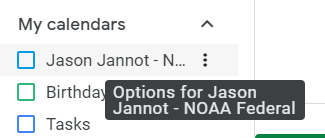
\includegraphics{_img/_gcalendar/pic1.png}

\begin{enumerate}
\def\labelenumi{\arabic{enumi}.}
\setcounter{enumi}{1}
\tightlist
\item
  Click settings and sharing
\end{enumerate}

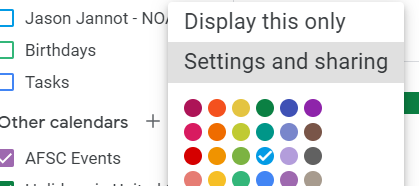
\includegraphics{_img/_gcalendar/pic2.png}

\begin{enumerate}
\def\labelenumi{\arabic{enumi}.}
\setcounter{enumi}{2}
\tightlist
\item
  Make sure to check ``Make available for National Oceanic and
  Atmospheric Administration'' and select ``See all event details'' in
  the drop down.
\end{enumerate}

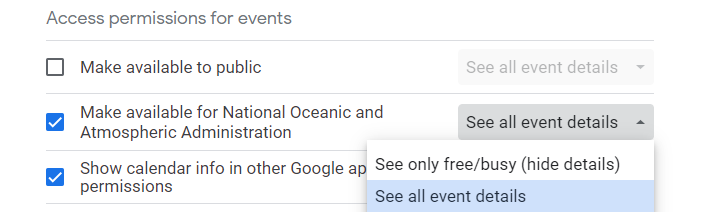
\includegraphics{_img/_gcalendar/pic3.png}

That should do it.

\chapter{Acronyms}\label{sec-acronyms}

The US Government is absolutely slaphappy about acronyms.

\begin{longtable}[]{@{}
  >{\raggedright\arraybackslash}p{(\columnwidth - 2\tabcolsep) * \real{0.3889}}
  >{\raggedright\arraybackslash}p{(\columnwidth - 2\tabcolsep) * \real{0.6111}}@{}}
\toprule\noalign{}
\begin{minipage}[b]{\linewidth}\raggedright
\textbf{Acronym}
\end{minipage} & \begin{minipage}[b]{\linewidth}\raggedright
\textbf{Definition}
\end{minipage} \\
\midrule\noalign{}
\endhead
\bottomrule\noalign{}
\endlastfoot
AFSC & Alaska Fisheries Science Center \\
AKRO & Alaska Regional Office \\
AMMOP & Alaska Marine Mammal Observer Program \\
A-Team & FMA Analytical Services Program \\
BSAI & Bering Sea Aleutian Islands \\
CAC & Common Access Card, a.k.a., your ``ID badge'' \\
DD & Division Director \\
FMA & Fisheries Monitoring and Analysis Division \\
FMAC & Fishery Monitoring Advisory Committee \\
GOA & Gulf of Alaska \\
M-Team & FMA Management Team = DD, Deputy Director, Debriefing PM,
Training PM, Analytical Services PM \\
NPFMC & North Pacific Fishery Management Council \\
NPOP & North Pacific Observer Program \\
OOO & Out Of Office \\
PCFMAC & Partial Coverage Fishery Monitoring Committee \\
PM & Program Manager \\
PSMFC & Pacific States Marine Fisheries Commission (colloquially,
PacStates) \\
SON & Statement of Nondisclosure for Using Confidential Fisheries
Data \\
WRC & Western Regional Center, a.k.a., the Sand Point Seattle Campus \\
\end{longtable}

\chapter{References}\label{references}

\phantomsection\label{refs}
\begin{CSLReferences}{1}{0}
\bibitem[\citeproctext]{ref-wilson2017}
Wilson, Greg, Jennifer Bryan, Karen Cranston, Justin Kitzes, Lex
Nederbragt, and Tracy K. Teal. 2017. {``Good Enough Practices in
Scientific Computing.''} Edited by Francis Ouellette. \emph{PLOS
Computational Biology} 13 (6): e1005510.
\url{https://doi.org/10.1371/journal.pcbi.1005510}.

\end{CSLReferences}

\chapter{Contributing}\label{contributing}

\chapter{How to Contribute}\label{how-to-contribute}

This document describes how to contribute to this project.

\begin{itemize}
\tightlist
\item
  Great to have you here.
\item
  You can help make this project better!
\item
  Thank you for your efforts.
\end{itemize}

\section{Code of Conduct}\label{code-of-conduct}

This project and everyone participating in it is governed by the
\href{https://sites.google.com/noaa.gov/myafsc/home/about-afsc}{AFSC
Code of Conduct} as well as the
\href{https://nmfs-opensci.github.io/GitHub-Guide/}{Github and Git
Guidance and Best Practices for NMFS Users}. By contributing to this
project you agree to abide by these terms.

\section{Team members}\label{team-members}

\textbf{Lead}: Jason E. Jannot, NOAA Fisheries AFSC FMA Division,
Seattle, WA.

\textbf{Contributors}:

\begin{itemize}
\item
  Jennifer Cahalan, Pacific States Marine Fisheries Commission and AFSC
  FMA Division, Seattle, WA
\item
  Craig Faunce, NOAA Fisheries AFSC FMA Division, Seattle, WA
\item
  Christian Gredzens, NOAA Fisheries AFSC FMA Division, Seattle, WA
\item
  Andy Kingham, NOAA Fisheries AFSC FMA Division, Seattle, WA
\item
  Geoff Mayhew, NOAA Fisheries AFSC FMA Division, Seattle, WA
\item
  Cameron Van Horn, Pacific States Marine Fisheries Commission and AFSC
  FMA Division, Seattle, WA
\end{itemize}

\section{Getting Started}\label{getting-started}

\begin{itemize}
\tightlist
\item
  Make sure you have a GitHub account.
\item
  Clone the repository from GitHub to your local machine.
\item
  Questions? email jason.jannot@noaa.gov
\end{itemize}

\section{Git Workflow for
Collaborating}\label{git-workflow-for-collaborating}

A Git workflow is a recommendation for how to use Git to accomplish work
in a consistent and productive manner. The goals is that the workflow
enhances the effectiveness of the team and does not limit productivity.
A good workflow proactively reduces the number of merge conflicts and
merges that need to be reverted. The choice of workflow by a team should
be a joint decision. Jason's recommendation is to use the
\href{https://www.atlassian.com/git/tutorials/comparing-workflows/gitflow-workflow}{GitFlow}
workflow because it accomplishes two important, but somewhat competing,
tactics to reduce merge conflicts when collaborating with git:

\begin{enumerate}
\def\labelenumi{\arabic{enumi}.}
\item
  \textbf{Branch life should be minimized} The risk of merge conflicts
  increase in proportion to the time the branch has been separate from
  the main branch. Short-lived branches promote cleaner merges.
\item
  \textbf{Branches should be tested before merging} Testing a branch
  before merging into the main branch reduces problems. However,
  accidents happen, thus a good workflow allows for easy reverts that
  don't cause issues for other contributors.
\end{enumerate}

\emph{Having said all that, I welcome all discussions on how to best
develop our Git workflow!} - Jason.

For those interested a comparison of Git workflows can be found
\href{https://www.atlassian.com/git/tutorials/comparing-workflows}{here}.

\section{Data}\label{data-1}

No PII or BII data or data that could identify fishers, individual
fishing locations, or individual processors should be saved to this
repository. Any such data will be removed immediately. For further
guidance see: \href{https://nmfs-opensci.github.io/GitHub-Guide/}{Github
and Git Guidance and Best Practices for NMFS Users}.

\section{Fixing typos}\label{fixing-typos}

You can fix typos, spelling mistakes, or grammatical errors in the
documentation directly using the GitHub web interface, as long as the
changes are made in the \emph{source} file. This generally means you'll
need to edit
\href{https://roxygen2.r-lib.org/articles/roxygen2.html}{roxygen2
comments} in an \texttt{.R}, not a \texttt{.Rd} file. You can find the
\texttt{.R} file that generates the \texttt{.Rd} by reading the comment
in the first line.

\section{Bigger changes}\label{bigger-changes}

If you want to make a bigger change, it's a good idea to first file an
issue and make sure someone from the team agrees that it's needed. If
you've found a bug, please file an issue that illustrates the bug with a
minimal \href{https://www.tidyverse.org/help/\#reprex}{reprex} (this
will also help you write a unit test, if needed). See the tidyverse
guide on \href{https://code-review.tidyverse.org/issues/}{how to create
a great issue} for more advice. Other sources for issue best practices
are described in various places on the web, such as
\href{https://medium.com/nyc-planning-digital/writing-a-proper-github-issue-97427d62a20f}{here}
and
\href{https://rewind.com/blog/best-practices-for-using-github-issues/}{here}.

\section{Making Changes}\label{making-changes}

The following uses the Gitflow method as the workflow.

\begin{itemize}
\tightlist
\item
  Clone the package onto your computer. If you haven't done this before,
  we recommend using
  \texttt{usethis::create\_from\_github("jjannot-NOAA/AnnualReportADPGantt",\ fork\ =\ TRUE)}.
\item
  Pull the most recent code.
\item
  Create a Git branch for your pull request (PR). We recommend using
  \texttt{usethis::pr\_init("brief-description-of-change")}.
\item
  Make your changes.
\item
  Commit your changes. See the \hyperref[git-commit-messages]{Git Commit
  Messages} styleguide below.
\item
  Push your changes to the remote Github repository.
\item
  Go to Github and create a `pull request' e.g., by running
  \texttt{usethis::pr\_push()}, and following the prompts in your
  browser. The title of your PR should briefly describe the change.See
  the \hyperref[pull-requests-messages]{Pull Requests Messages} section
  below.
\item
  Assign a reviewer.
\end{itemize}

\section{Styleguides}\label{styleguides}

\subsection{Git Commit Messages}\label{git-commit-messages}

As a general rule, you should commit when you finish something that
allows your code to work - usually ends up being a couple times an hour.

\begin{itemize}
\tightlist
\item
  Use the present tense (``Add feature'' not ``Added feature'')
\item
  Use the imperative mood (``Move cursor to\ldots{}'' not ``Moves cursor
  to\ldots{}'')
\item
  Limit the first line to 72 characters or less
\item
  Reference issues and pull requests liberally after the first line
\end{itemize}

\subsection{Pull Requests Messages}\label{pull-requests-messages}

For general guidelines, please see
\href{https://docs.github.com/en/pull-requests/collaborating-with-pull-requests/proposing-changes-to-your-work-with-pull-requests/creating-a-pull-request}{Github's
Pull Request} page.

In the message, please include the following headers:

\begin{itemize}
\tightlist
\item
  Description of the Issue or New Feature
\item
  Description of What Has Been Done
\item
  Usage

  \begin{itemize}
  \tightlist
  \item
    Examples and/or how others might test the change
  \end{itemize}
\item
  Assign a Reviewer - this will most likely be the Merge Master. In the
  case of the Merge Master, this will be another appropriate
  contributor.
\end{itemize}

\subsection{Coding conventions}\label{coding-conventions}

Start reading our code and you'll get the hang of it. We optimize for
readability.

\begin{itemize}
\item
  Scripts should not be longer than 400-600 lines.
\item
  We use \href{https://cran.r-project.org/package=roxygen2}{roxygen2},
  with
  \href{https://cran.r-project.org/web/packages/roxygen2/vignettes/rd-formatting.html}{Markdown
  syntax}, for documentation.
\item
  Never use \texttt{rm(list\ =\ ls())} Why, you ask? Well first off,
  Jenny Bryan is likely to come
  \href{https://www.tidyverse.org/blog/2017/12/workflow-vs-script/}{set
  your computer on fire}. More specifically, it mixes \emph{your}
  workflow (i.e., personal choices) with \emph{the} product (i.e., the R
  code needed by someone else to run your code). See Jenny's in-depth
  discussion at the link above.
\item
  Write functions. There's a good chance that your script can be
  simplified into a function. ``Everything that happens is a function
  call.'' - John Chambers
\item
  Always put spaces after list items and method parameters (1, 2, 3, not
  1,2,3) and around operators (x + y = 1, not x+y=1).
\item
  Eliminate unnecessary white space. I realize this conflicts with the
  previous statement, but I'm comfortable with that ambiguity.
\item
  Use a styler and IDE to keep your code clean.
  \href{https://styler.r-lib.org/}{\texttt{stylr}} is a good R package
  for keeping your code tidy and easy to use.
\item
  \texttt{tidyverse} methods, especially those using pipes,
  \texttt{\%\textgreater{}\%}, increase readability and make reviewing
  code much more pleasant.
\item
  When in doubt, consult the
  \href{https://style.tidyverse.org/}{\texttt{tidyverse} style guide}
\end{itemize}

This is collaborative software. Consider the people who will read your
code, and make it look nice for them. It's sort of like driving a car:
Perhaps you love doing donuts when you're alone, but with passengers the
goal is to make the ride as smooth as possible.

\subsection{File structure and
conventions}\label{file-structure-and-conventions}

Keeping a tidy project requires maintaining order amongst files.

\begin{itemize}
\item
  General folder structure is:

  \begin{itemize}
  \tightlist
  \item
    -- root

    \begin{itemize}
    \tightlist
    \item
      -- data
    \item
      -- figures
    \item
      -- notes
    \item
      -- R
    \item
      -- scripts
    \item
      -- tables
    \item
      -- tests (optional)
    \end{itemize}
  \end{itemize}
\item
  root directory in addition to holding the folders (above), should only
  contain configuration and R package files.
\item
  data - holds any data files used in the project.
\item
  figures - holds any figure files created by the project.
\item
  notes - holds \texttt{TODO.Rmd}, \texttt{Notes.Rmd},
  \texttt{SCRATCH.R/.Rmd} and reusable templates (for Roxygenating
  functions, headers for commenting code) or example code. The
  \texttt{TODO.Rmd} is being worked on and what has recently been done
  and should closely mirror Git commits. \texttt{Notes.Rmd} is more
  narrative than \texttt{TODO} and contains important information that
  is too detailed/complex for a vignette. Scratch files are sandboxes
  for working out code.
\item
  R - should hold only functions. Each function should be called
  \texttt{\textless{}my-special-function-name\textgreater{}\_function.R}.
\item
  scripts - these are the scripts that run the analysis. Each script
  name should start with a number in the order the scripts are to be
  run. The first script in the sequence is typically
  \texttt{0\_Setup.R}. \texttt{Setup.R} sets the paths for the project
  (this makes it reproducible on your machine!), loads all necessary
  libraries, date constants, functions, and data. The next script in the
  sequence might be, e.g., \texttt{1\_Pre\_Processing.R}, followed by
  \texttt{2\_Data\_Wrangling.R}, \texttt{3\_Analysis.R},
  \texttt{4\_Plots.R}\ldots note: these are just examples.
\item
  tables - holds any tables generated by the scripts.
\item
  tests - any unit tests that might be applicable. This is optional.
\end{itemize}

\section{Reviewing Pull Requests}\label{reviewing-pull-requests}

\begin{itemize}
\tightlist
\item
  Open the pull request
\item
  Review the code changes
\item
  Reviewer - provide comments and feedback in GitHub
\item
  Originator - respond to comments, perhaps add comments
\item
  Approve changes (upper right corner) and add approval comment
\item
  \textbf{Merge Master/Code owner merges all pull requests! Please do
  not merge your own pull request.} If the Merge Master is pushing code,
  then the reviewer should be responsible for merging the pull request.
\item
  MergeMaster will delete the branch once the code has been merged.
\item
  \textbf{DONT FORGET TO PULL the new code} to your local instance to
  get latest code.
\end{itemize}

\begin{itemize}
\tightlist
\item
  If you have further questions, contact: Jason Jannot
  jason.jannot@noaa.gov
\end{itemize}



\end{document}
